\documentclass[a4paper,10pt]{article}
\pdfpagewidth
\paperwidth
\pdfpageheight
\paperheight
\usepackage[english]{babel}
\usepackage[utf8]{inputenc}
\usepackage[babel]{csquotes}    %per biblatex
\usepackage[sorting=none,]	%mettere per ordinare secondo l'ordine di chiamata
{biblatex}   %bibliografia
\usepackage{epsfig}
\usepackage{fancyhdr} 
\usepackage{amsmath,amssymb}
\RequirePackage{fix-cm}		%per il comando successivo
\DeclareMathSizes{10}{10}{5}{4}		%regola la size dei pedici: testo, testo, pedice, subpedice
\usepackage{amscd} 
\usepackage[T1]{fontenc} 
\usepackage[usenames,dvipsnames]{xcolor}
\usepackage{graphicx,color,listings}
\graphicspath{{../fig/}}	%percorso per le immagini
\usepackage{placeins}   %per \floatbarrier
\usepackage{hologo}
\frenchspacing
\usepackage{rotating}
\usepackage[bf,small]{caption}	%pacchetto caption
\captionsetup{tableposition=top,figureposition=bottom,font=small}
\usepackage{textcomp, gensymb}  %textcomp è per usare %, ° e altri simboli
\usepackage{hyperref}	%tutti i tipi di collegamento tranne vref
\hypersetup{colorlinks=true,	%attiva colori
 linkcolor=red,	%ref
 filecolor=black,
 urlcolor=blue,		%url
 citecolor=green,		%cite
 pdftitle={DNA model}	%per citare questo pdf?
}
\usepackage{multirow}
%\usepackage{multicol}  %per scrivere su più colonne
%\setlength{\columnsep}{10mm}	%spazio fra le colonne
\usepackage{picture}
\usepackage{booktabs}
%\usepackage{subfig}	%per subfigure all'interno dello stesso ambiente figure
\usepackage{subcaption}
\usepackage{float}  %per [H]
%\usepackage{circuitikz}    %circuiti
\usepackage[separate-uncertainty=true]{siunitx} %unità di misura
\usepackage{newlfont}
\usepackage{setspace}   %interlinee diverse
\usepackage[version=4]{mhchem}  %formule chimiche
\usepackage[english]{varioref}  %referenze che espicitano la pagina
\usepackage{geometry}	%margini: già se presente li cambia
% \geometry{
%   left=15mm,
%   top=20mm,
%   right=15mm,
%   bottom=20mm,
% }

\bibliography{bib}

\title{DNA coars-grain elastic model to reproduce characteristics of higher-order structures\thanks{Chiral selection in wrapping, crossover, and braiding of DNA mediated by asymmetric bend-writhe elasticity\cite{main}}}
\author{Tommaso Rondini\thanks{Master's degree student in Physics, University of Bologna (Italy). Email: tommaso.rondini@studio.unibo.it}}

\begin{document}
\maketitle

\section*{Abstract}
In a paper of the $2015$~\cite{main}, Tomohiro Yanao, Sosuke Sano and Kenichi Yoshikawa have improved their previously model~\cite{old, very_old} of the DNA double helix structure.
They have implemented this model to analyse wrapping, crossover, and braiding of DNA, phenomenons of fundamental interest on genome packaging, gene regulation, and enzyme recognition.
The study has explored elastic mechanisms for the selection of these processes of DNA based on a coarse-grained model.

The DNA model consists of two elastic chains that mutually intertwine in a right-handed manner forming a double-stranded helix with the distinction between major and minor grooves.
Although individual potential energy functions of the DNA model have no asymmetry in terms of left and right twist, the model as a whole exhibits an asymmetric propensity to writhe in the left direction upon bending due to the right-handed helical geometry.
Monte Carlo simulations of this model suggest that DNA has a propensity to prefer left-handed wrapping around a spherical core particle and also around a uniform rod due to the asymmetric elastic coupling between bending and writhing.
This result indicates an elastic origin of the uniform left-handed wrapping of DNA in nucleosomes and also has implications on the wrapping of double-stranded DNA around rod-like molecules.
Monte Carlo simulations of the DNA model also suggest that two juxtaposed DNA molecules can braid each other spontaneously under moderate attractive interactions with the preference for left-handed braiding due to the asymmetric coupling between bending and writhing.
This result suggests the importance of asymmetric elasticity in the selection of chirality in braiding of a pair of DNA molecules.

I have recreated the simulations to check their results.
The main aspects of the study have been achieved: the DNA model prefers left-handed writhing and braiding and the distributions of the parameters reflect the expected ones.
Some differences happen, maybe due to statistical issues and to a complex landscape potential.

\section{Introduction}
Higher-order structures of DNA are the subject of extensive studies for their significance in genome packaging, gene regulation, and enzyme recognition~\cite{1,2}.
Wrapping, crossover, and braiding are among the most fundamental and essential higher-order structures of DNA.
Since all these higher-order structures are associated with superhelical conformations of DNA, chirality, i.e., right- or left-handedness, of these superhelical motifs should play important roles.
This study thereby has explored a possible mechanism for the selection of chirality in wrapping, crossover, and braiding of DNA based on a coarse-grained elastic model.
Since not only DNA but also many other biopolymers assume helical conformations, roles of helical chirality are of rather universal interest~\cite{3}.

In eukaryotic DNA achieves a highly compact and hierarchical packaging in a cell nucleus, which is called chromatin~\cite{10}.
At the lowest level of the hierarchy of chromatin, DNA wraps around a protein core particle called histone octamer about $1.75$ times in a left-handed manner~\cite{1,2}.
The uniform left-handedness of this wrapping should be important for the clustering of nucleosomes mediated by charge distributions~\cite{16} to form further higher-order structures in chromatin.
The present study has tried to develop a minimal model to account for the stability of left-handed wrapping of DNA around a core particle in terms of asymmetric elasticity of DNA.
In addition to wrapping of DNA around a core particle, wrapping and unwrapping of DNA around rod-like molecules~\cite{27}, including carbon nanotubes~\cite{rod_2}, is also an interesting subject.
The present study also has addressed the issue of chirality of DNA adsorbed on a uniform rod.

Crossover and braiding are important motifs of DNA for genome packaging, gene regulation, and enzyme recognition~\cite{br_1}.
Some researches~\cite{br_1, br_2, br_3} had suggested that right-handed crossover is more stable than left-handed one in solution due to groove-backbone interaction especially in the presence of divalent cations.
Moreover, Kornyshev et al.~\cite{br_4, br_5} had suggested that braiding of DNA molecules could be driven by electrostatic interactions and that left-handed braiding is preferred over right-handed one due to helical alignment.
It is clear that right-handed crossover implies left-handed braiding and vice-versa.
This study has explored the roles of mechanical interaction for the selection and stability of left-handed braiding of DNA in terms of the intrinsic asymmetric elasticity, or nonlinear coupling, between bending and writhing of DNA, as the intrinsic property of helical double-stranded polymer.

\section{Model of Double-Stranded DNA}
\subsection{Coordinates of the DNA model}
The model of DNA in that study consists of two elastic chains intertwining around a central backbone.
The central backbone is a chain with the same number of element as the bases chains.
The position of the $i$ element is given by a three dimensional vector $\textbf{r}_i \ \left(i=1,\dots ,N\right)$.
The distance between adjacent nodal point is $b = 0.34$\si{\nm}, which is the distance between to neighbouring base pairs.
The first node is set at some coordinates (now we assume that it is $(0,\ 0,\ 0)^T$);
the z-axis is in the direction of the second node, the y-axis lies in the plain made by the first three nodes and the x-axis is perpendicular to the z and y axis, creating a right-hand system.
In this way, the position of the second node is $(0,\ 0,\ b)^T$ in the reference system of the first node.
We assign a three-dimension orthonormal frame $F_i$ to each node (it is useful for set the position of the bases): in each $i$-th system the z-axis is an extension to the link between the $\left (i-1\right )$-th and the $i$-th node, the y-axis lies in the plain formed by $\textbf{r}_{i-1},\ \textbf{r}_i$ and $\textbf{r}_{i+1}$, and $\hat{x}_i=\hat{y}_i\times\hat{z}_i$.
Now we see that $F_2=F_1$.
We introduce angles $\Theta_2$ that rotate the $\hat{x}_2$-axis so that $\hat{z}_3$ is parallel to the link between the third and the second node.
We have to define $\Theta_i$ angles with $i=2,\dots,N-1$.
The fourth frame $F_4$ y-axis lies in a different plane, so we have to introduce dihedral angles $\Phi_i\ (i=2,\dots,N-2)$ to rotate around $\hat{z}_3$.
So we have:
\begin{equation}\label{eq:c_coo}
\textbf{r}_i=\textbf{r}_{i-1}+\textbf{R}^{2}_{3}\left(\Phi_1,\Theta_2\right)\textbf{R}^{3}_{4}\left(\Phi_2,\Theta_3\right)\dots\textbf{R}^{i-1}_{i}\left(\Phi_{i-2},\Theta_{i-1}\right)\textbf{b}\qquad (i=3,\dots,N)
\end{equation}
where $\textbf{b}=(0,\ 0,\ b)^T$, $\Phi_1=0\degree$, and
\begin{equation}\label{eq:r_matrix}
\textbf{R}^{i-1}_{i}\left(\Phi_{i-2},\Theta_{i-1}\right)=
\begin{pmatrix}
\cos\Phi_{i-2} & -\sin\Phi_{i-2} & 0 \\
\sin\Phi_{i-2} & \cos\Phi_{i-2} & 0 \\
0 & 0 & 1 \\
\end{pmatrix}
\begin{pmatrix}
1 & 0 & 0 \\
0 & \cos\Theta_{i-1} & -\sin\Theta_{i-1} \\
0 & \sin\Theta_{i-1} & \cos\Theta_{i-1} \\
\end{pmatrix}
\end{equation}

The two chains of the model represent the two sugar-phosphate chains of DNA.
The bonds between adjacency sugar-phosphate elements are elastic, as harmonic springs.
Their positions are represented by $\textbf{P}_i$ and $\textbf{Q}_i$ respectively.
The distance between the backbone structure and the DNA chains is fixed to $\sigma_0=1.0$\si{\nm}, and $p_{i}$ and $q_{i}$ elements are linked with a rigid rod that is the hydrogen-bonded base pair.
We introduce $\psi_i\ (i=1,\dots,N)$ that is the internal twist angle characterizing the relative orientation of $i$-th base pair with respect to $i$-th frame attached to the central backbone;
and $\omega_0$ is the common constant angle between the two vectors $\textbf{P}_i-\textbf{r}_i$ and $\textbf{Q}_i-\textbf{r}_i$.
So the positions $\textbf{p}_i$ and $\textbf{q}_i$ respect to $\textbf{r}_i$ are
\begin{equation}
\begin{split}
\textbf{p}_i & =\left(\sigma_0\cos\psi_i,\ \sigma_0\sin\psi_i,\ 0\right)^T \qquad (i=1,\dots,N) \\
\textbf{q}_i & =\left(\sigma_0\cos\left(\psi_i+\omega_o\right),\ \sigma_0\sin\left(\psi_i+\omega_0\right),\ 0\right)^T \qquad (i=1,\dots,N)
\end{split}
\end{equation}
Instead, their absolute positions are: $\textbf{P}_1=\textbf{p}_1$, $\textbf{Q}_1=\textbf{q}_1$, $\textbf{P}_2=\textbf{r}_2-\textbf{p}_2$, $\textbf{Q}_2=\textbf{r}_2-\textbf{q}_2$,
\begin{equation}
\textbf{P}_i=\textbf{r}_i-\textbf{R}^{2}_{3}\left(\Phi_1,\Theta_2\right)\textbf{R}^{3}_{4}\left(\Phi_2,\Theta_3\right)\dots\textbf{R}^{i-1}_{i}\left(\Phi_{i-2},\Theta_{i-1}\right)\textbf{p}_i\qquad (i=3,\dots,N)
\end{equation}
\begin{equation}
\textbf{Q}_i=\textbf{r}_i-\textbf{R}^{2}_{3}\left(\Phi_1,\Theta_2\right)\textbf{R}^{3}_{4}\left(\Phi_2,\Theta_3\right)\dots\textbf{R}^{i-1}_{i}\left(\Phi_{i-2},\Theta_{i-1}\right)\textbf{q}_i\qquad (i=3,\dots,N)
\end{equation}
Thus, when $\psi_i$ changes, the nodal points $\textbf{P}_i$ and $\textbf{Q}_i$ move together.
$\Theta_i$, $\Phi_i$ and $\psi_i$ are the conformation parameters of this model.

Fig.~\ref{fig:model_a} shows the conformation of the DNA molecule with $N=5$ and little perturbation of $\Theta_{i}\ \left (i = 1,\dots,4\right )$ and $\Phi_{i}\ \left (i = 1,\dots,3\right )$.
Since the central backbone was been created just to construct the coordinates and has not any direct influence on the configuration energy, from now on in the figures we will not show it.

\begin{figure}[tb]
\centering
\begin{subfigure}{.4\textwidth}
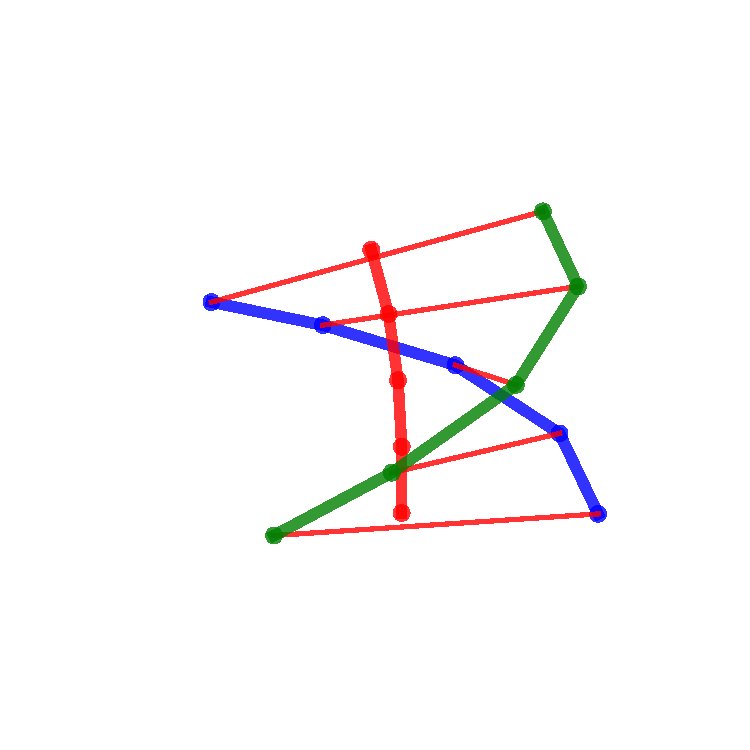
\includegraphics[width=\textwidth]{main_5.pdf}
\caption{$N=5$}
\label{fig:model_a}
\end{subfigure}
\begin{subfigure}{.4\textwidth}
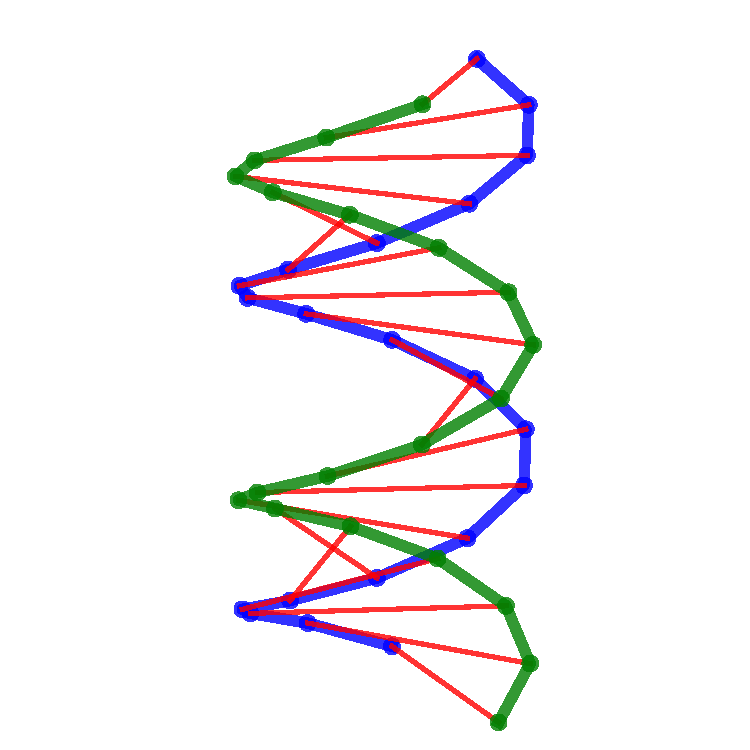
\includegraphics[width=\textwidth]{main_20.pdf}
\caption{$N=20$}
\label{fig:model_b}
\end{subfigure}
\caption{(a) Graphical visualization of the DNA model with $N=5$ and different $\Theta$ and $\Phi$. (b) Graphical visualization of the DNA model with $N=20$ and $\Theta=\Phi=0\degree$.}
\label{fig:model}
\end{figure}

\subsection{Equilibrium conformation}
For the equilibrium conformation they have assumed that the central backbone takes a straight conformation (e.g. $\Theta_i=0\degree\ (i=2,\dots,N-1)$ and $\Phi_i=0\degree\ (i=2,\dots,N-2)$.
They have assumed that the two sugar-phosphate chains complete one helical cycle per every $10$ nodal points as in B-form DNA~\cite{1, 2}.
Thus, at the equilibrium conformation the angle between two neighbouring nodal points is $\psi_0=36\degree$ with respect to the central backbone when vertically projected onto the plane perpendicular to the central backbones.
As a result, the pitch of each helical turn of the double-strand is \SI{3.4}{\nm}.

The internal twist angle $\psi_i$ is so set to
\begin{equation}
\psi_i=\left(i-1\right) \psi_0
\end{equation}
In order to make the width of major groove \SI{2.2}{\nm} and that of minor groove \SI{1.2}{\nm} at the equilibrium conformation~\cite{1, 2} they assume that the constant angle $\omega_0$ to be
\begin{equation}
\omega_0=1.2\text{nm}\times\dfrac{360\degree}{3.4\text{nm}}\simeq127.06\degree
\end{equation}
Based on the above settings, the equilibrium length of each elastic bond between consecutive nodal points is
\begin{equation}\label{eq:l_0}
\ell_0=\sqrt{2\sigma_0^2\left(1-\cos\psi_0\right)+b^2}\simeq0.705\text{nm}
\end{equation}
and the equilibrium bending angle at each nodal point is
\begin{equation}\label{eq:theta_0}
\theta_0=\cos^{-1}\left[\dfrac{2\sigma_0^2\left(1-\cos\psi_0\right)\cos\psi_0+b^2}{2\sigma_0^2\left(1-\cos\psi_0\right)+b^2}\right]\simeq31.4\degree
\end{equation}
Fig.~\ref{fig:model_b} shows the conformation of the DNA molecule with $N=20$ and $\Theta_{i}=\Phi_{i}=0\degree$.
The red lines represent the hydrogen-bonds between the two sugar-phosphate chains (green and blue).
The major and the minor grooves can be seen.

\subsection{Energy functions}
Here I introduce the essential energy functions for general double-stranded helical chains.
They are bonding and bending energy of the P- and Q-chain.
The total bonding energy is given by
\begin{equation}\label{eq:bond}
V_{bond}=\sum_{i=1}^{N-1}\dfrac{1}{2}k_{bond}\left(\left|\textbf{P}_{i+1}-\textbf{P}_{i}\right|-\ell_0\right)^2+\sum_{i=1}^{N-1}\dfrac{1}{2}k_{bond}\left(\left|\textbf{Q}_{i+1}-\textbf{Q}_{i}\right|-\ell_0\right)^2
\end{equation}
where $\ell_0$ has been determined in Eq.~\ref{eq:l_0} and $k_{bond}$ is the bonding rigidity.
The total bending energy is given by
\begin{equation}\label{eq:bend}
V_{bend}=\sum_{i=2}^{N-1}\dfrac{1}{2}k_{bend}\left(\theta_i^{(P)}-\theta_0\right)^2+\sum_{i=2}^{N-1}\dfrac{1}{2}k_{bend}\left(\theta_i^{(Q)}-\theta_0\right)^2
\end{equation}
where $\theta_0$ has been determined in Eq.~\ref{eq:theta_0} and $k_{bend}$ is the bending rigidity.
$\theta_i^{(P)}$ and $\theta_i^{(Q)}$ are the bending angles in the P- and Q-chains respectively and are given by~\cite{old}
\begin{equation}
\begin{split}
\theta_i^{(P)} & =\cos^{-1}\left(\dfrac{\textbf{P}_{i}-\textbf{P}_{i-1}}{\left|\textbf{P}_{i}-\textbf{P}_{i-1}\right|}\cdot\dfrac{\textbf{P}_{i+1}-\textbf{P}_{i}}{\left|\textbf{P}_{i+1}-\textbf{P}_{i}\right|}\right)\qquad \left(i=2,\dots,N-1\right) \\
\theta_i^{(Q)} & =\cos^{-1}\left(\dfrac{\textbf{Q}_{i}-\textbf{Q}_{i-1}}{\left|\textbf{Q}_{i}-\textbf{Q}_{i-1}\right|}\cdot\dfrac{\textbf{Q}_{i+1}-\textbf{Q}_{i}}{\left|\textbf{Q}_{i+1}-\textbf{Q}_{i}\right|}\right)\qquad \left(i=2,\dots,N-1\right)
\end{split}
\end{equation}

The two rigidity parameters can not be found directly by experiments.
To evaluate them, they have taken experimental data and assume that the energy is a quadratic function of the bending angles and have set the parameters since they reproduce as better as they can the quadratic function.
The estimated parameters are
\begin{equation}
k_{bond}=1000\text{pN/nm}\qquad k_{bend}=7000\text{pNnm}
\end{equation}

\subsection{Monte Carlo algorithm}
They have used the Metropolis Monte Carlo algorithm to incorporate the effects of thermal and noisy environments.
Suppose that we have a ``current'' conformation of the DNA model with total energy $V$.
Then, we randomly choose one angle between all the bending ($\Theta_i$), dihedral ($\Phi_i$) and twist ($\psi_i$) angles and perturb it by $\pm1\degree$ randomly to obtain a ``trial'' conformation with energy $V_{tr}$.
If the trial conformation has a lower energy ($V_{tr}<V$), the trial conformation is accepted.
If the trial conformation has a higher energy ($V_{tr}>V$), we accept the trial conformation with the probability
\begin{equation}\label{eq:prob}
p=\exp{\left(-\dfrac{V_{tr}-V}{k_{B}T}\right)}
\end{equation}
with temperature set to $T=$\SI{300}{\kelvin}

Note that the Monte Carlo algorithm of the present study uses only these three kinds of angles, $\Theta$, $\Phi$, and $\psi$, as mentioned above for making trial movements.
This makes it possible to highlight the roles of the coupling between bending and writhing of the DNA model.
On the other hand, however, this algorithm can limit the movements of other degrees of freedom of the DNA model.

\section{Results}
\subsection{Asymmetric bend-writhe elasticity of the DNA model}\label{sec:bend_writh}
In this section I study the fundamental elasticity of the DNA model with particular attention to the coupling between bending and writhing of the central backbone.
Fig.~\ref{fig:bend}(a)-(c) show the conformations of the DNA model. where all dihedral angles are set to $\Phi_i=-4\degree$ and all bending angles are set to $\Theta_i=1\degree$ in Fig.~\ref{fig:bend_a}, $\Theta_i=3\degree$ in Fig.~\ref{fig:bend_b}, and $\Theta_i=5\degree$in  Fig.~\ref{fig:bend_c}.
Fig.~\ref{fig:bend}(d)-(f) show the same bending angles but dihedral angles are set to $\Phi_i=+4\degree$.
From these figures, we confirm that negative dihedral angles $\Phi_i$ give rise to left-handed super-helical conformations, while positive dihedral angles $\Phi_i$ give rise to right-handed super-helical conformations.
We also see that the more bending angles $\Theta_i$ increase, the more super-helical pitch of the DNA model decreases and super-helical radius increases, under conditions of fixed dihedral angles $\Phi_i$.

\begin{figure}[tb]
\centering
\begin{subfigure}{0.3\textwidth}
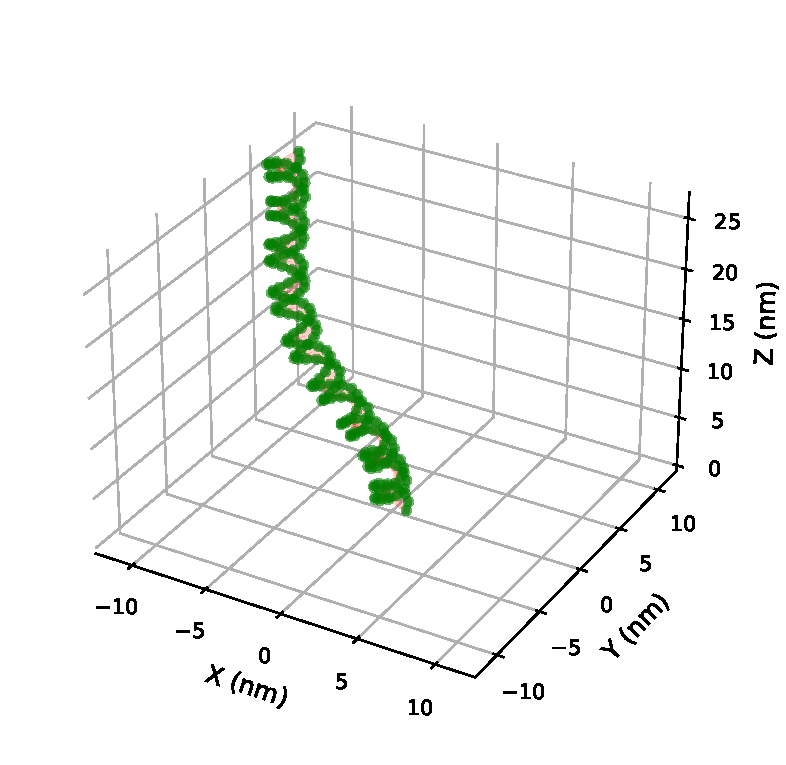
\includegraphics[width=\textwidth]{bw_-4_1.pdf}
\caption{$\Phi=-4\degree,\ \Theta=1\degree$}
\label{fig:bend_a}
\end{subfigure}
\begin{subfigure}{0.3\textwidth}
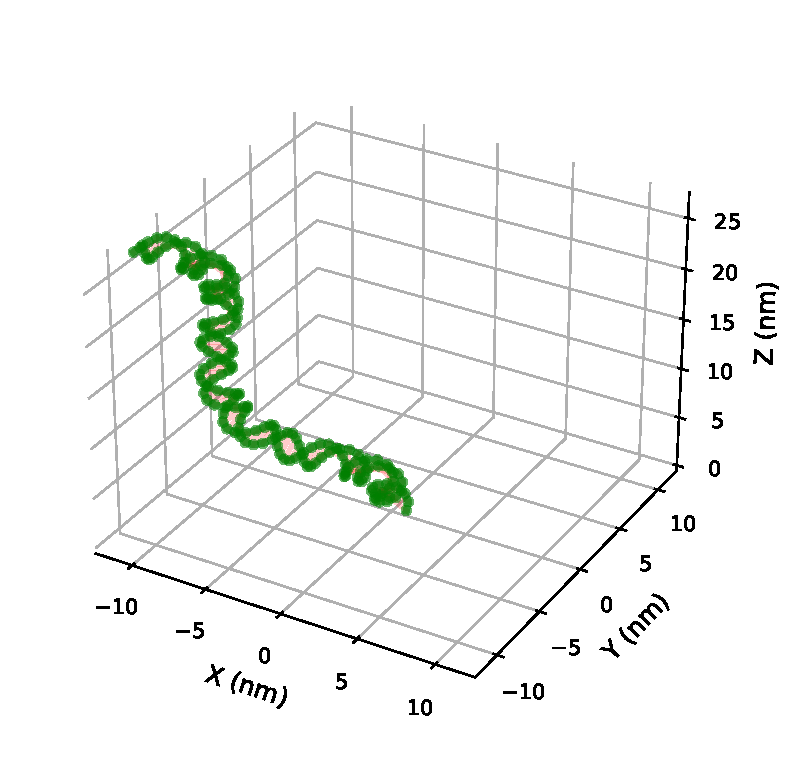
\includegraphics[width=\textwidth]{bw_-4_3.pdf}
\caption{$\Phi=-4\degree,\ \Theta=3\degree$}
\label{fig:bend_b}
\end{subfigure}
\begin{subfigure}{0.3\textwidth}
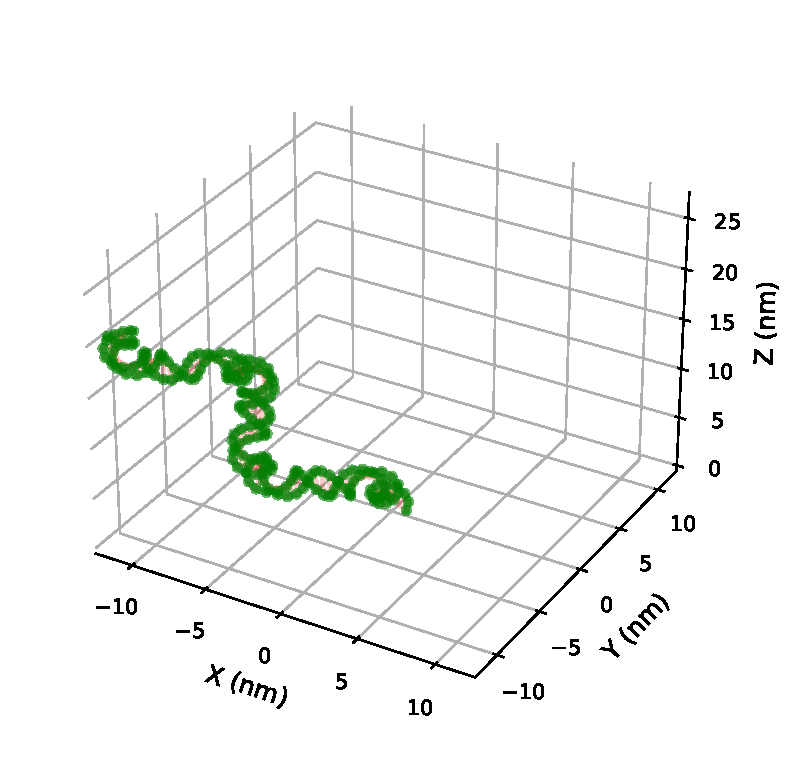
\includegraphics[width=\textwidth]{bw_-4_5.pdf}
\caption{$\Phi=-4\degree,\ \Theta=5\degree$}
\label{fig:bend_c}
\end{subfigure}
\begin{subfigure}{0.3\textwidth}
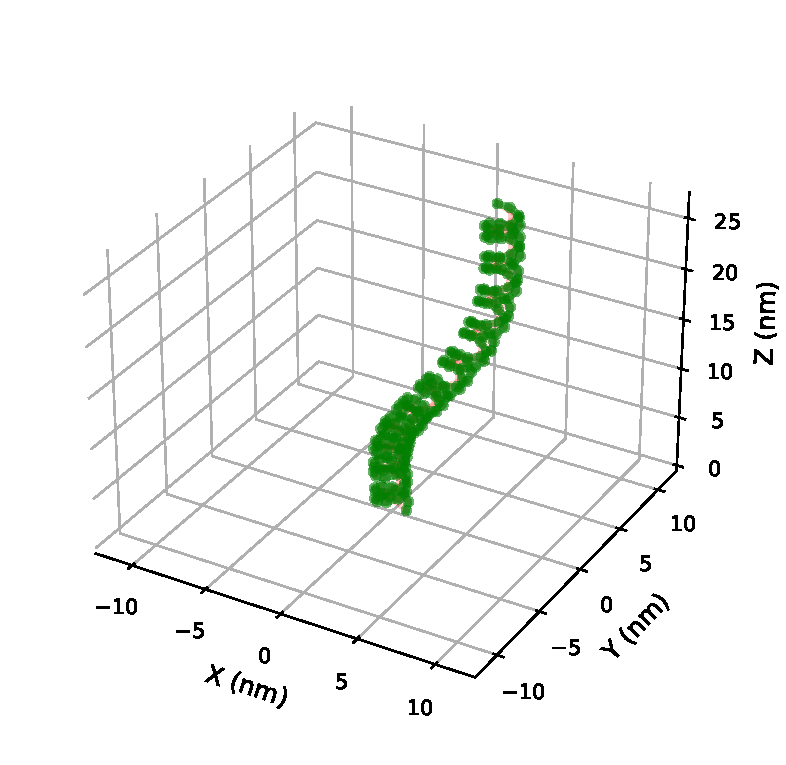
\includegraphics[width=\textwidth]{bw_4_1.pdf}
\caption{$\Phi=4\degree,\ \Theta=1\degree$}
\label{fig:bend_d}
\end{subfigure}
\begin{subfigure}{0.3\textwidth}
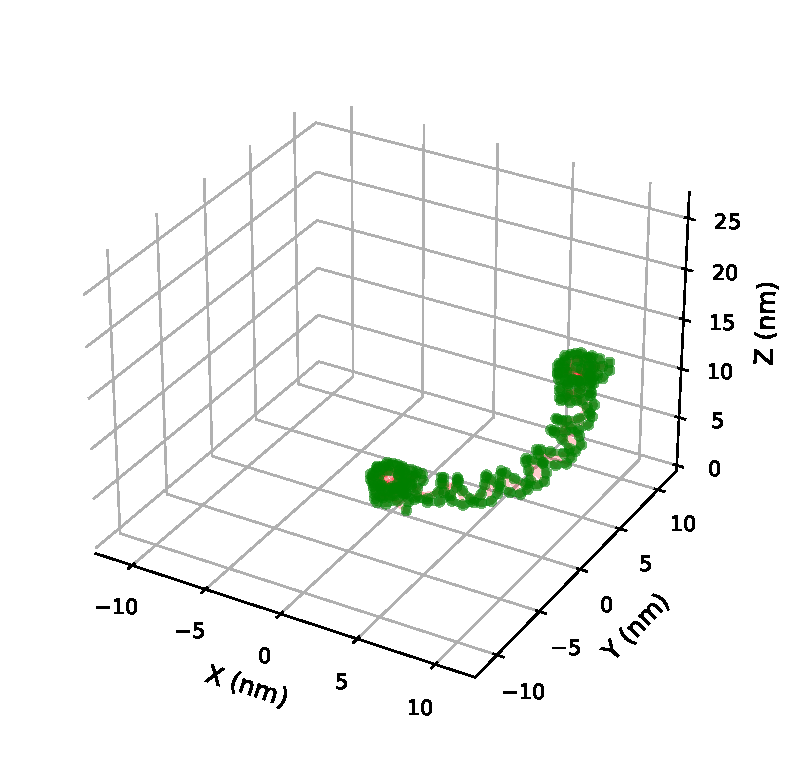
\includegraphics[width=\textwidth]{bw_4_3.pdf}
\caption{$\Phi=4\degree,\ \Theta=3\degree$}
\label{fig:bend_e}
\end{subfigure}
\begin{subfigure}{0.3\textwidth}
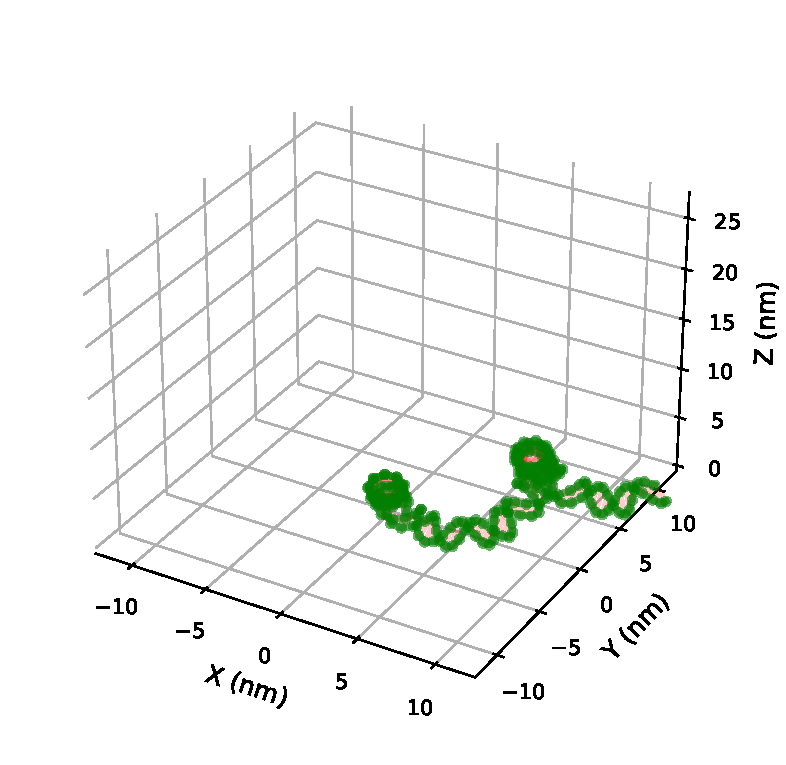
\includegraphics[width=\textwidth]{bw_4_5.pdf}
\caption{$\Phi=4\degree,\ \Theta=5\degree$}
\label{fig:bend_f}
\end{subfigure}
\caption{Conformation to the DNA model with $N=100$ base pairs for all the combination between dihedral angles ($\Phi=\pm 4\degree$) and bending angles ($\Theta=$\SIlist{1;3;5}{\degree}).}
\label{fig:bend}
\end{figure}

Fig.~\ref{fig:bend_energy} shows the dependence of the total energy of the DNA mode with $N=100$ nodes, $V_{DNA}=V_{bond}+V_{bend}$ defined by Eq.~\ref{eq:bond} and Eq.~\ref{eq:bend} on writhing the central backbone.
All the dihedral angles are set to the same value $\Phi$ that changes from $-4\degree$ to $4\degree$, while all bending angles are fixed to $1\degree$ (solid curve, blue), $3\degree$ (broken curve, green), and $5\degree$ (dash-dotted curve, red).
There is an evident asymmetry between left-handed writhing ($\Phi<0$) and right-handed writhing ($\Phi>0$).
In particular left-handed writhing has a lower energy value at the same absolute value of dihedral angle, and increasing bending angles this difference increases.
This result clearly indicates the intrinsic asymmetric coupling between bending and writhing of the DNA model.
Specifically, the DNA model has a preference for left-handed writhing upon bending.
The asymmetric bend-writhe elasticity observed in Fig.~\ref{fig:bend_energy} should be the result of the right-handedness of the double-stranded model of DNA since there is no other chirality in the model or in the potential energy functions of the DNA model.

\begin{figure}[tb]
\centering
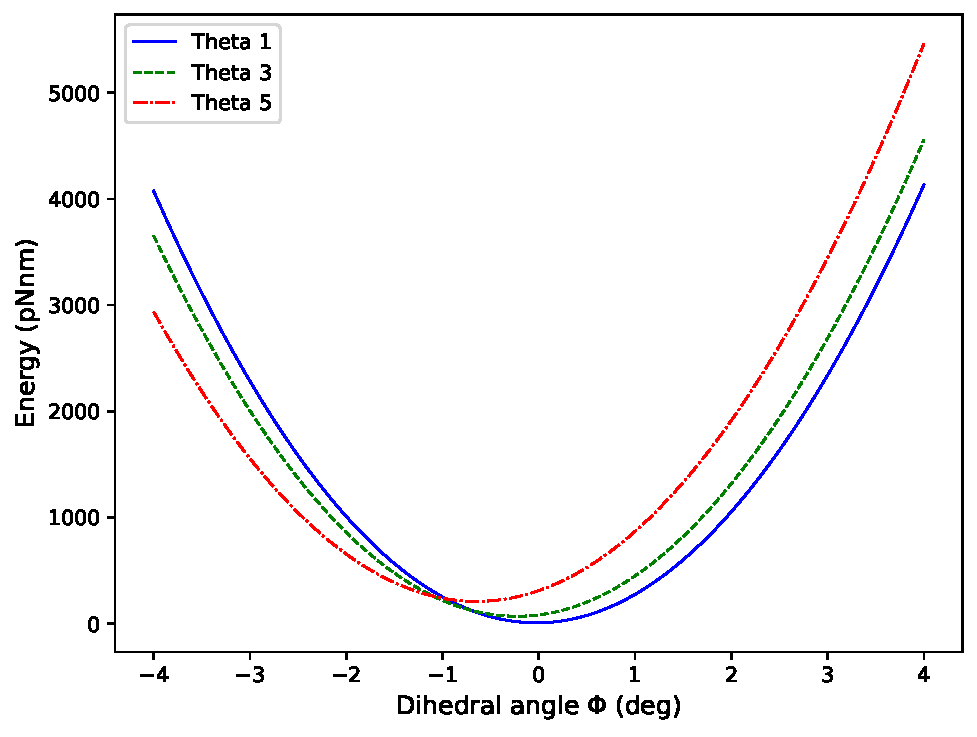
\includegraphics[width=.5\textwidth]{bw_energy.pdf}
\caption{Dependence of total energy of the DNA model with $N=100$ nodes, on the writhe of the central backbone, i.e., the value of dihedral angles.
Each line is the total energy at different bending angles.
All dihedral and bending angles are equal for all the nodes.
The solid blue curve has $\Theta=1\degree$.
The green broken curve has $\Theta=3\degree$.
The dashed-dotted red curve has $\Theta=5\degree$.}
\label{fig:bend_energy}
\end{figure}

\subsection{Chiral selection in wrapping of the DNA model around a spherical core particle}\label{sec:core}
The asymmetric bend-writhe elasticity observed in Sec.~\ref{sec:bend_writh} indicates that DNA may have a preference on the directionality, i.e., chirality, in wrapping around a core particle.
This is a useful test because in a nucleosome, DNA usually wraps around histone octamer about 1.75 times in a left-handed manner~\cite{1, 2}.
In this section I try to account for the stability of the left-handed wrapping of DNA around a core particle in terms of the asymmetric elasticity of the DNA model, using the same parameters of the paper.

In the Monte Carlo simulation they have used a Morse potential instead of electrostatic one for the attraction between DNA and core particle, since it requires less machine time.
The potential is
\begin{equation}\label{eq:core}
V_{core}=\sum_{i=1}^{N}D_{core}\left\{\exp\left[-2\beta_{core}\left(\left|\textbf{r}_{i}-\textbf{r}_{core}\right|-\sigma_{core}\right)\right]-2\exp\left[-\beta_{core}\left(\left|\textbf{r}_{i}-\textbf{r}_{core}\right|-\sigma_{core}\right)\right]\right\}
\end{equation}
where $\textbf{r}_i$ is the position of the $i$-th nodal point of the central backbone and $\textbf{r}_{core}$ is the position of the center of the spherical core.
$\sigma_{core}=$ \SI{4.5}{\nm} is the equilibrium distance between the center of the core and each nodal point of the central backbone, $\beta_{core}=$ \SI{2.0}{\per\nm} determines the width of the Morse potential, and $D_{core}=$ \SI{10}{\pico\newton\nano\meter} determines the strength of the interaction.

To avoid overlaps of the DNA with itself, they  have introduced a potential for the excluded volume effect (it is the repulsive part of the Morse potential)
\begin{equation}\label{eq:exc}
V_{exc}=\sum_{i=1}^{N-n}\sum_{j=i+n}^{N}D_{exc}\exp\left[-2\beta_{exc}\left(\left|\textbf{r}_{i}-\textbf{r}_{j}\right|-\sigma_{exc}\right)\right]
\end{equation}
where they have set $\beta_{exc}=$ \SI{2.0}{\per\nm}, $\sigma_{exc}=$ \SI{2.1}{\nm}, and $D_{exc}=$ \SI{1.0}{\pico\newton\nano\meter}.
The parameter $n=7$ removes the repulsions between very close nodal points in comparison to $\sigma_{exc}$.

I have performed Monte Carlo simulation for a DNA model with $N=200$ nodes, where the position of the first two base pairs and of the core are fixed.
The total energy function used to perform the Metropolis algorithm with Eq.~\ref{eq:prob} now is
\begin{equation}\label{eq:hist_energy}
V=V_{bond}+V_{bend}+V_{core}+V_{exc}
\end{equation}

Fig.~\ref{fig:hist} show some of the results of Monte Carlo simulations, where $\textbf{r}_{core}=\left(0,\ -4.5,\ 10.2\right)^T$ in unit of \si{\nm}.
We see DNA wrapping around the histone in a left-handed manner up to about $2$ turns.

\begin{figure}[tb]
\centering
\begin{subfigure}{.3\textwidth}
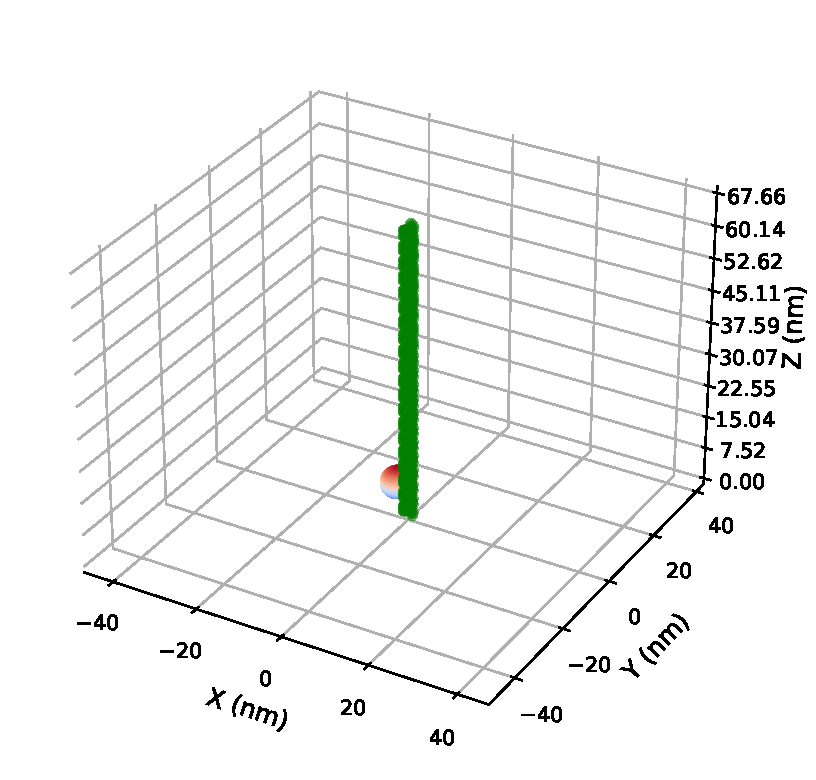
\includegraphics[width=\textwidth]{hist_0.pdf}
\caption{0th step}
\label{fig:hist_a}
\end{subfigure}
\begin{subfigure}{.3\textwidth}
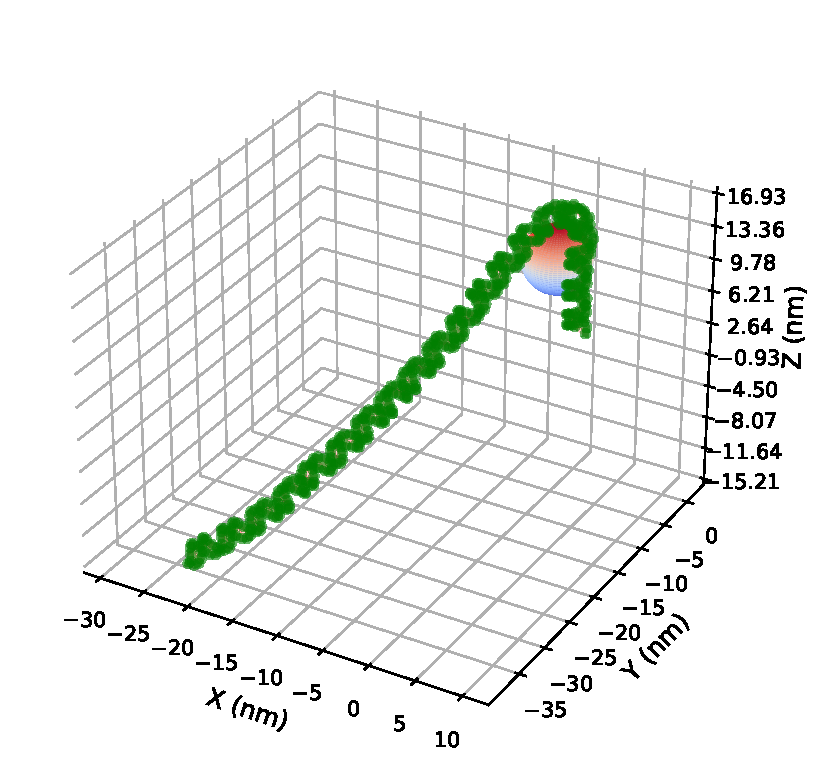
\includegraphics[width=\textwidth]{hist_100000.pdf}
\caption{100000th step}
\label{fig:hist_b}
\end{subfigure}
\begin{subfigure}{.3\textwidth}
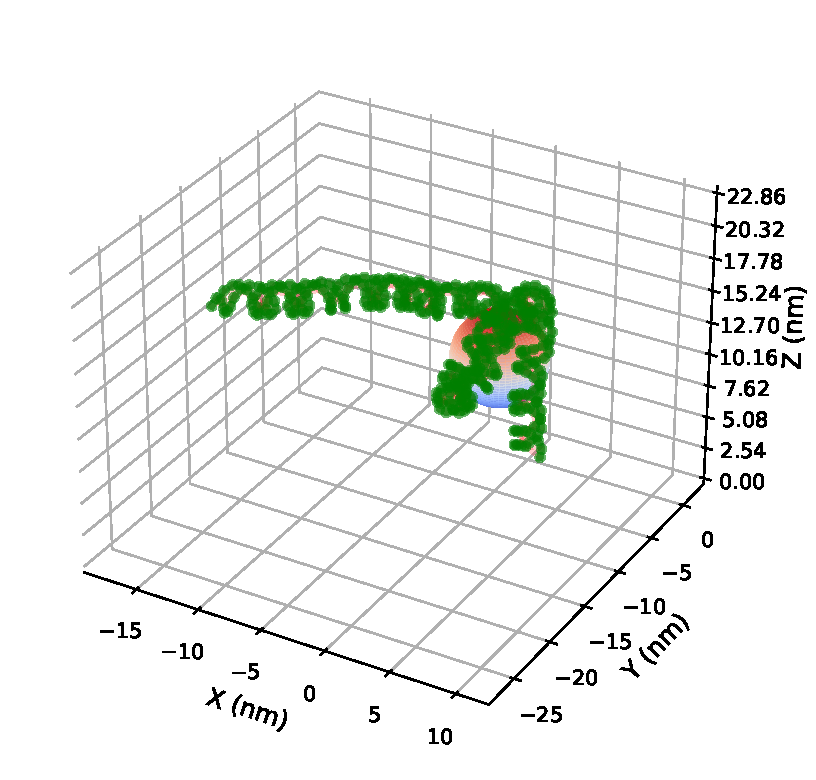
\includegraphics[width=\textwidth]{hist_300000.pdf}
\caption{300000th step}
\label{fig:hist_c}
\end{subfigure}
\begin{subfigure}{.3\textwidth}
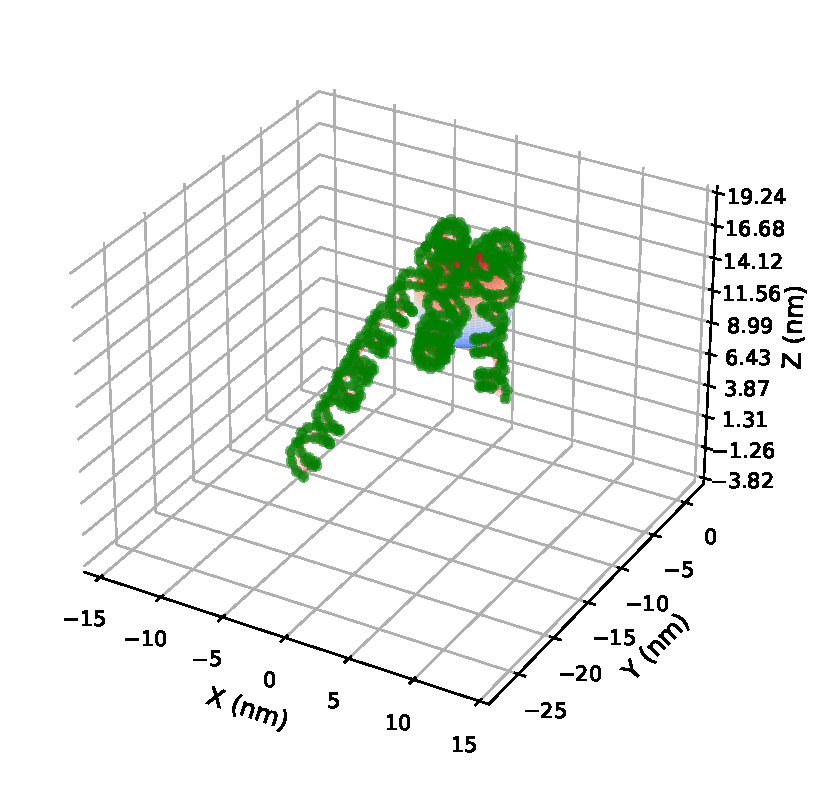
\includegraphics[width=\textwidth]{hist_400000.pdf}
\caption{400000th step}
\label{fig:hist_c2}
\end{subfigure}
\begin{subfigure}{.3\textwidth}
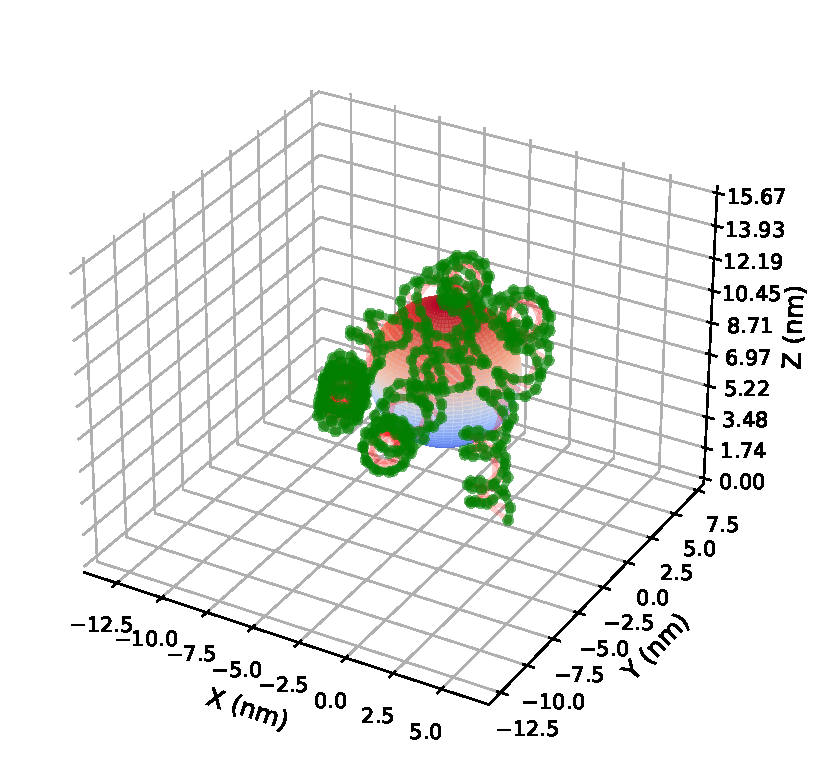
\includegraphics[width=\textwidth]{hist_500000.pdf}
\caption{500000th step}
\label{fig:hist_c3}
\end{subfigure}
\begin{subfigure}{.3\textwidth}
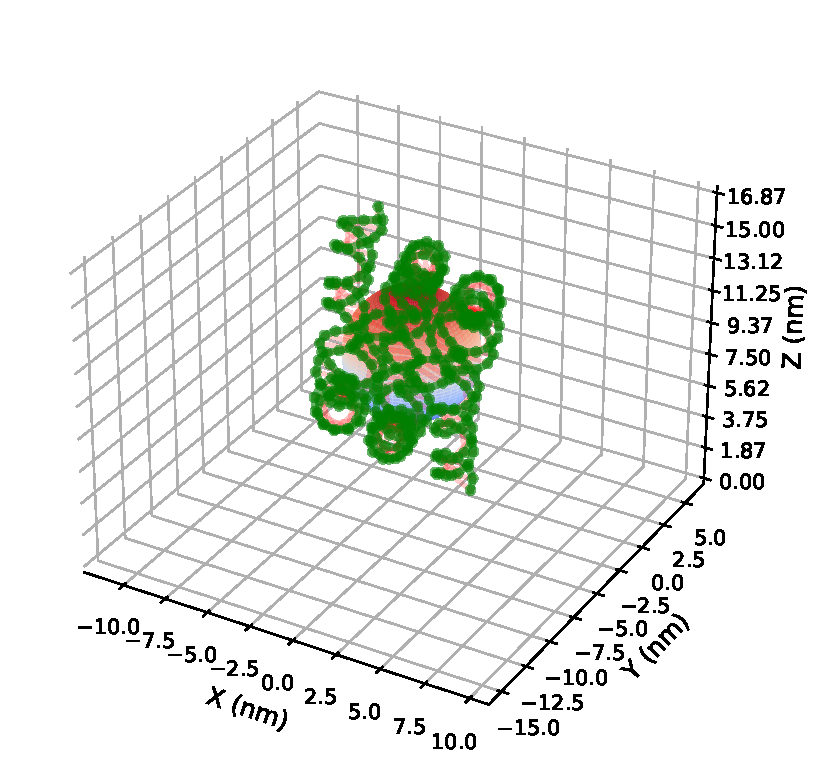
\includegraphics[width=\textwidth]{hist_600000.pdf}
\caption{600000th step}
\label{fig:hist_d}
\end{subfigure}
\caption{Monte Carlo simulation for wrapping of the DNA model with $N=200$ nodes around a spherical core particle at \SIlist{0;100000;300000;600000}{} step.}
\label{fig:hist}
\end{figure}

Fig.~\ref{fig:hist_en} shows the evolution of the total energy: we see as energy tends to decrease and equilibrate as the DNA wraps around the core, except for the initial abrupt increase.
Fig.~\ref{fig:hist_wr} shows the corresponding evolution of wrapping number~\cite{very_old} defined by
\begin{equation}\label{eq:wrap_num}
W=\dfrac{b\left(N_{ad}-1\right)}{2\pi\sigma_{core}}
\end{equation}
where $N_{ad}$ is the number of nodal points of the DNA model adsorbed on the core; they have assumed that a node is adsorbed if satisfies $\left|\textbf{r}_i-\textbf{r}_{core}\right|\leq$ \SI{4.8}{\nm}.
We see that the wrapping number increases as DNA wraps and equilibrates at around $W=1.75$.
In order to judge the chirality of the wrapping in a systematic manner, they have utilized chirality parameter~\cite{very_old} defined by
\begin{equation}\label{eq:chirality}
C=\langle\textbf{m}_{i}\rangle_{ad}\cdot\left(\langle\textbf{r}_{i}\rangle_{tail}-\langle\textbf{r}_{i}\rangle_{head}\right)
\end{equation}
where $\langle\textbf{m}_{i}\rangle_{ad}$ is obtained by averaging the vectors $\textbf{m}_i=\left(\textbf{r}_{i}-\textbf{r}_{i-1}\right)\times\left(\textbf{r}_{i+1}-\textbf{r}_{i}\right)$ over all adsorbed nodes and then normalizing it.
$\langle\textbf{r}_{i}\rangle_{head}$ represents the average of position vectors of the first half (with smaller subscripts $i$) of the adsorbed nodal points of the central backbone of DNA, whereas $\langle\textbf{r}_{i}\rangle_{tail}$ represents the average of position vectors of the last half (with larger subscripts $i$) of the adsorbed nodal points of the central backbone.
Positive sign of $C$ signifies right-handed wrapping while negative sign of $C$ signifies left-handed wrapping.
Fig.~\ref{fig:hist_ch} shows the evolution of the chirality parameter, and we see that $C$ takes mostly negative values.
Fig.~\ref{fig:hist_ch_pr} is the probability distribution of $C$ obtained from $10$ runs of Monte Carlo simulations, each of which consists of $6\times 10^5$ steps.
In order to avoid the bias due to the specific initial conditions introduced above, I have discarded the data of initial $3\times10^5$ steps from each Monte Carlo simulation.
The clear peak at negative value of $C$ indicates the strong propensity of the DNA model to wrap around the core in the left-handed manner.
The only negative values of $C$ indicates that in all the simulations the DNA wraps in left-handed manner around core particle.

\begin{figure}[tb]
\centering
\begin{subfigure}{.33\textwidth}
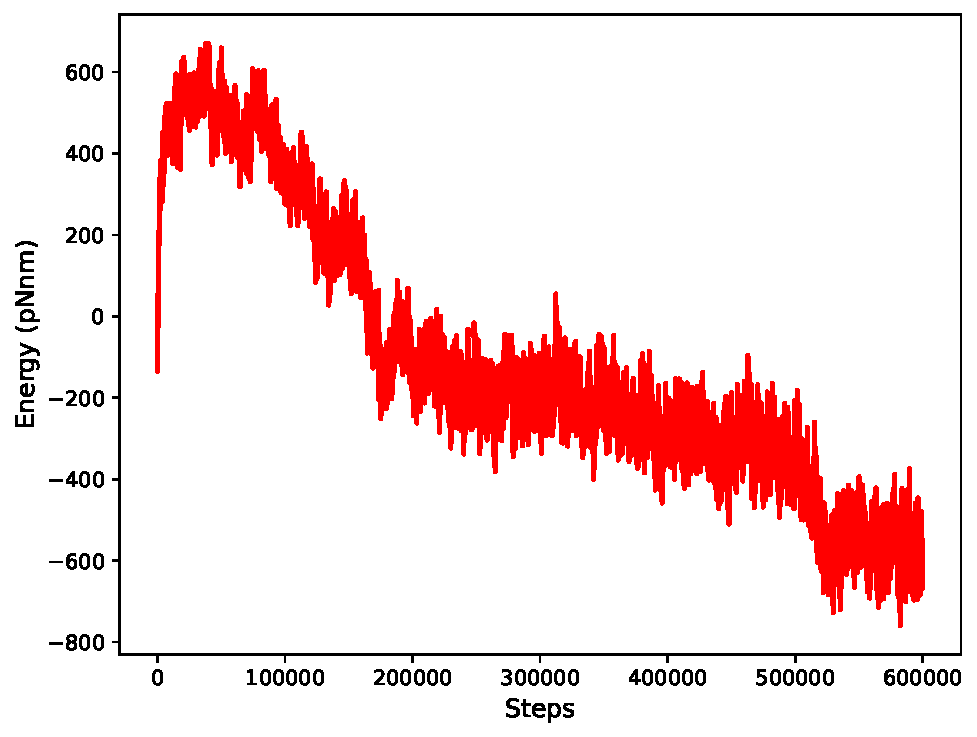
\includegraphics[width=\textwidth]{hist_energy.pdf}
\caption{}
\label{fig:hist_en}
\end{subfigure}
\begin{subfigure}{.33\textwidth}
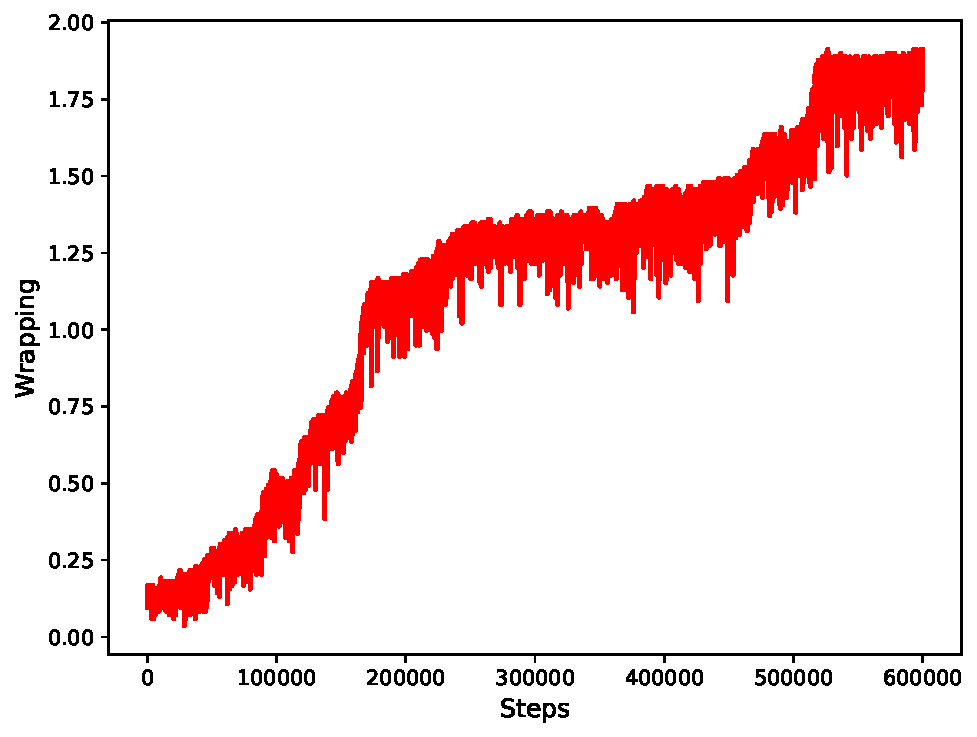
\includegraphics[width=\textwidth]{hist_wrapping.pdf}
\caption{}
\label{fig:hist_wr}
\end{subfigure}
\\
\begin{subfigure}{.33\textwidth}
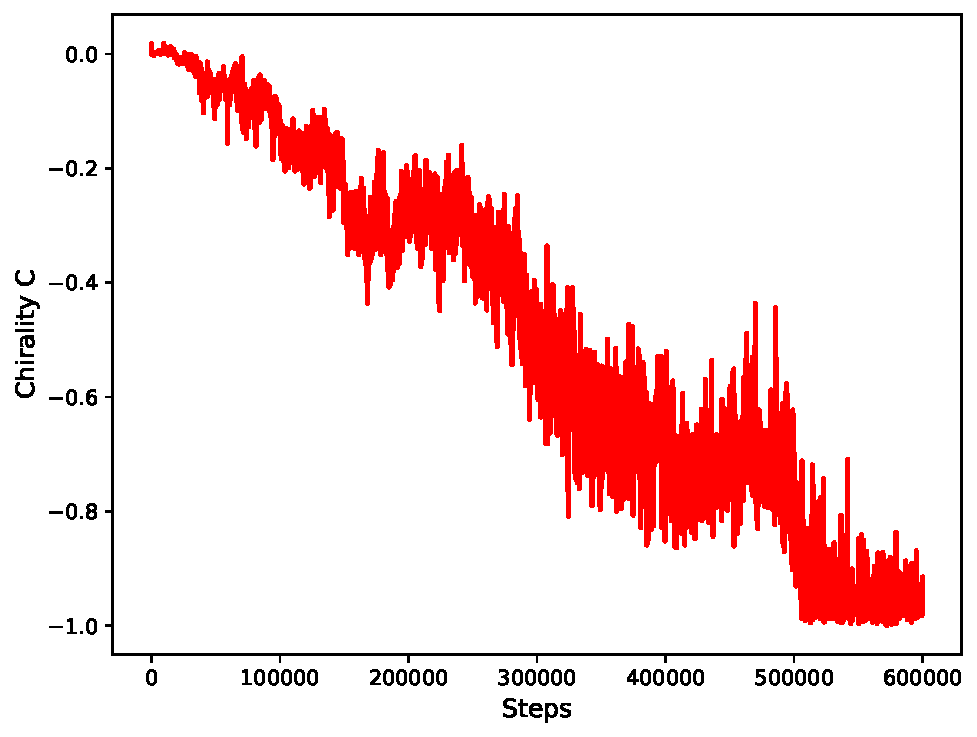
\includegraphics[width=\textwidth]{hist_chirality.pdf}
\caption{}
\label{fig:hist_ch}
\end{subfigure}
\begin{subfigure}{.33\textwidth}
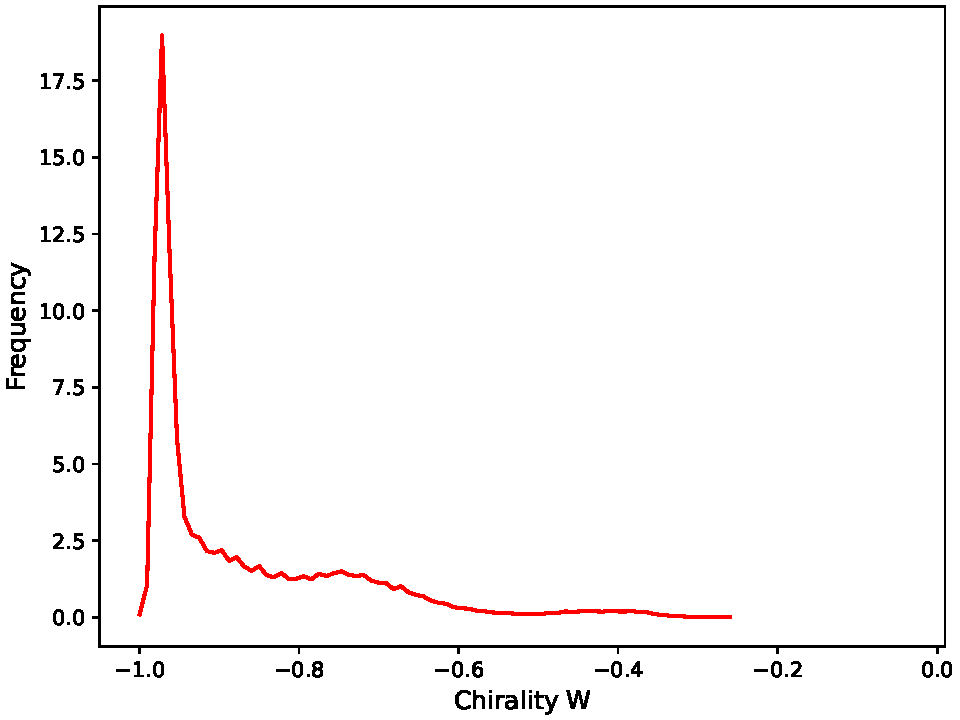
\includegraphics[width=\textwidth]{hist_ch_pr.pdf}
\caption{}
\label{fig:hist_ch_pr}
\end{subfigure}
\caption{(a) the evolution of total energy(Eq.~\ref{eq:hist_energy});
(b) the evolution of wrapping number (Eq.~\ref{eq:wrap_num});
(c) the evolution of chirality parameter (Eq.~\ref{eq:chirality});
(d) probability distribution of the chirality parameter obtained from $10$ runs of Monte Carlo simulation of $6\times 10^5$ steps without the first $3\times 10^5$.}
\label{fig:hist_params}
\end{figure}

\subsection{Chirality of the DNA model adsorbed on a uniform rod}\label{sec:rod}
Chiral selectivity of the DNA model observed in Sec.~\ref{sec:core} indicates that DNA may also exhibit chiral selectivity in wrapping around a uniform rod.
Indeed, conformation of DNA around rod-like molecules, such as carbon nanotube~\cite{rod_2}, is an interesting issue.
While wrapping of single-stranded DNA around carbon nanotubes is frequently studied, where wrapping geometry is known to be very sensitive to the DNA sequence~\cite{rod_1}, they have studied the chirality of the double-stranded DNA model adsorbed on a hypothetical uniform rod.

They have fixed the uniform rod so that the central axis of the rod coincides with the z-axis of the space.
They then have assumed an attractive interaction between DNA and the uniform rod using the Morse potential:
\begin{equation}\label{eq:rod_1}
V_{rod 1}=\sum_{i=1}^{N}D_{rod}\left\{\exp\left[-2\beta_{rod}\left(\sqrt{x_{i}^{2}+y_{i}^{2}}-\sigma_{rod}\right)\right]-2\exp\left[-\beta_{rod}\left(\sqrt{x_{i}^{2}+y_{i}^{2}}-\sigma_{rod}\right)\right]\right\}
\end{equation}
where $x_{i}$ and $y_{i}$ represent x- and y-components of the position vector of the central backbone of the DNA model.
$\sigma_{rod}$ determines the effective radius of the rod including the DNA radius.
They have examined three different values: \SIlist{2.1;3.1;4.1}{\nm}.
The parameter $D_{rod}=$ \SI{20}{\pico\newton\nano\meter} determines the strength of the interaction between rod and DNA, while $\beta_{rod}=$ \SI{2.0}{\per\nm} determines the width of the Morse potential.
Here they have used a DNA model with $N=100$ and introduce a excluded volume effect exactly the same as in Eq.~\ref{eq:exc}.
The total energy used to calculate probability (Eq.~\ref{eq:prob}) in the Monte Carlo simulations is
\begin{equation}\label{eq:rod_1_energy}
V=V_{bond}+V_{bend}+V_{rod 1}+V_{exc}
\end{equation}
The first nodal point of the central backbone is fixed to the space at $\left(\sigma_{rod},\ 0,\ 0\right )^T$.
The straight equilibrium conformation is thermally perturbed to take superhelical or undulating conformations around the rod.
They have introduced a wrapping number to characterize chirality and the number of wrapping
\begin{equation}\label{eq:wrap_rod}
W_{rod}=\dfrac{1}{2\pi}\sum_{i=2}^{N-1} sgn\left [\hat{\textbf{z}}\cdot\textbf{n}_{i}\right ]\cos^{-1}\left (\dfrac{x_{i}x_{i+1}+y_{i}y_{i+1}}{\sqrt{x_{i}^2+y_{i}^2}\sqrt{x_{i+1}^2+y_{i+1}^2}}\right )
\end{equation}
where $\hat{\textbf{z}}=\left (0,\ 0,\ 1\right )^T$, $\textbf{n}_i$ is a unit vector perpendicular to the central backbone at $i$-th node defined by  $\textbf{n}_i=\left (\textbf{r}_{i}-\textbf{r}_{i-1}\right )\times\left (\textbf{r}_{i+1}-\textbf{r}_{i}\right )/\left |\left (\textbf{r}_{i}-\textbf{r}_{i-1}\right )\times\left (\textbf{r}_{i+1}-\textbf{r}_{i}\right )\right |$, and $sgn\left [\right ]$ is the sign function.
Positive sign of $W_{rod}$ means right-handed wrapping of DNA around the rod, while negative sign means left-handed wrapping.
Absolute value of $W_{rod}$ can be regarded as a measure of the number of wrapping turns of the DNA model around the rod.

In Fig.~\ref{fig:r1} (down) the probability distribution of the wrapping number $W_{rod}$ is shown, obtained from $20$ runs of Monte Carlo simulations of the DNA model adsorbed on a uniform rod.
Each simulation is composed by $2\times 10^6$ steps, but the first $2\times 10^5$ are discarded in order to avoid the initial conditions dependences.
The rod radius parameter $\sigma_{rod}$ is \SI{2.1}{\nm} in Fig.~\ref{fig:r1_a}, \SI{3.1}{\nm} in Fig.~\ref{fig:r1_b}, and \SI{4.1}{\nm} in Fig.~\ref{fig:r1_c}.
We see that the distribution is almost symmetric for each $\sigma_{rod}$ value: this means that DNA model wraps equally in left and right way.
We see that the absolute value of the wrapping number tends to increase as the radius of the rod decreases.
Since $\left |W_{rod}\right |$ is mostly $<0.1$ we can see that the DNA model seldom wraps clearly around the rod.
In Fig.~\ref{fig:r1} (above) some images of the DNA segment with $N=100$ around rods of different diameter are shown.

\begin{figure}[tb]
\centering
\begin{subfigure}{.3\textwidth}
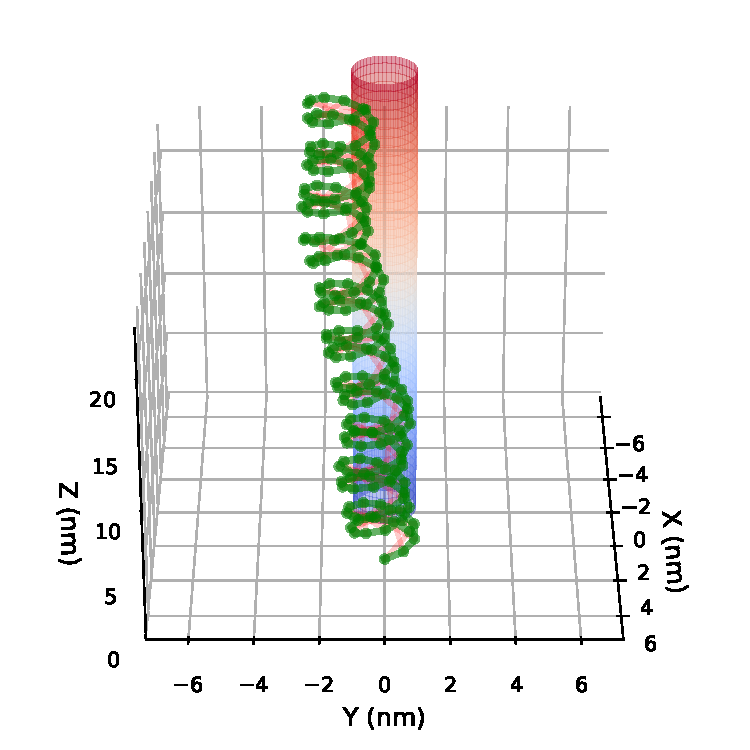
\includegraphics[width=\textwidth]{r1_A_2000000.pdf}
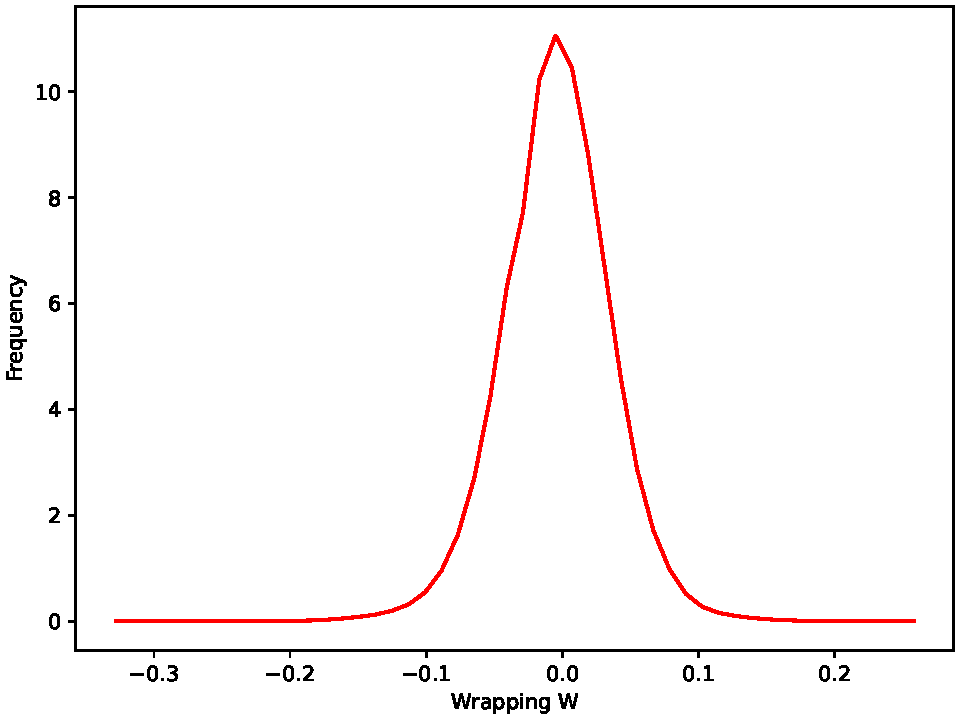
\includegraphics[width=\textwidth]{r1_A_wr_pr.pdf}
\caption{$\sigma_{rod}=$ \SI{2.1}{\nm}}
\label{fig:r1_a}
\end{subfigure}
\begin{subfigure}{.3\textwidth}
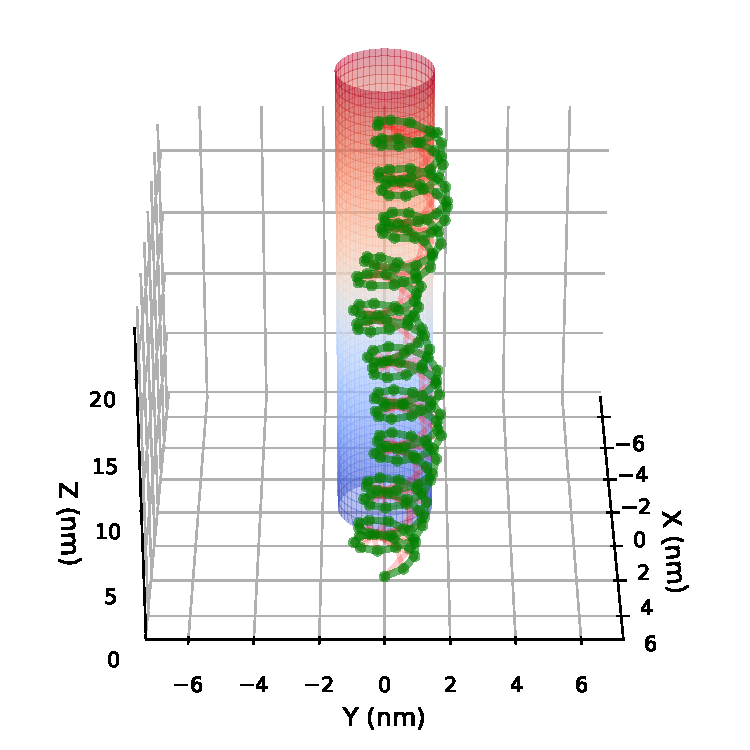
\includegraphics[width=\textwidth]{r1_B_2000000_17.pdf}
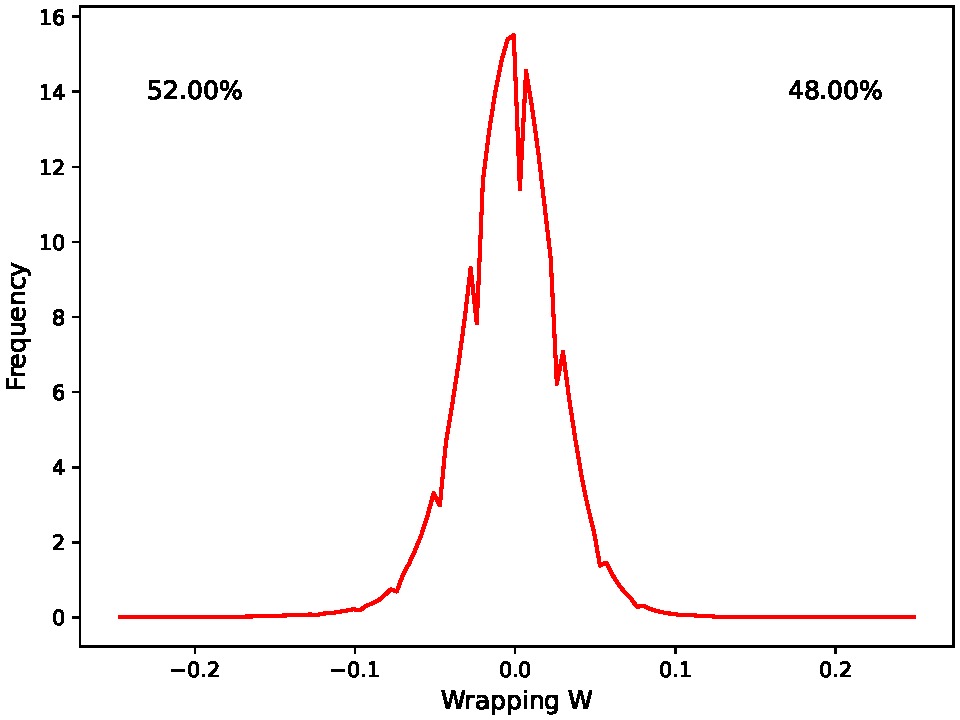
\includegraphics[width=\textwidth]{r1_B_wr_pr.pdf}
\caption{$\sigma_{rod}=$ \SI{3.1}{\nm}}
\label{fig:r1_b}
\end{subfigure}
\begin{subfigure}{.3\textwidth}
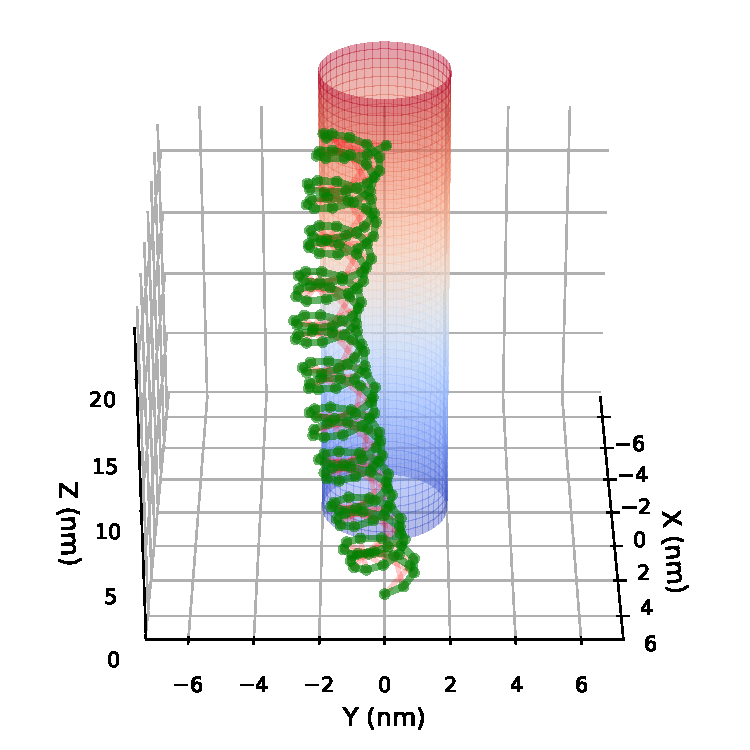
\includegraphics[width=\textwidth]{r1_C_2000000_7.pdf}
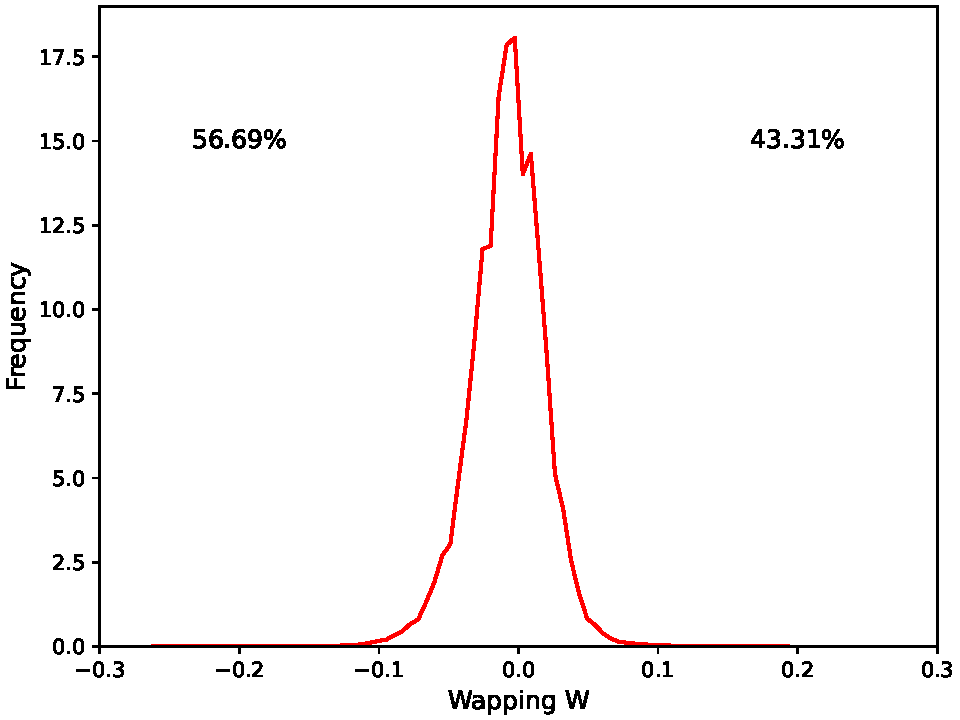
\includegraphics[width=\textwidth]{r1_C_wr_pr.pdf}
\caption{$\sigma_{rod}=$ \SI{4.1}{\nm}}
\label{fig:r1_c}
\end{subfigure}
\caption{Probability distribution of the wrapping number obtained from $20$ Monte Carlo simulations of $2\times 10^6$ steps (behind) and an example of the DNA wrapping model with $W_{rod}\simeq 0$ with $\sigma_{rod}=$ \SI{2.1}{\nm} (a), \SI{3.1}{\nm} (b), and \SI{4.1}{\nm} (c). The rod local potential was used (Eq.~\ref{eq:rod_1}).}
\label{fig:r1}
\end{figure}

On the other hand, when the attraction between DNA and a rod is ''global'', in the sense that a part of the rod attracts many different parts of DNA and a part of DNA attracts many different parts the rod, we will see that the symmetry is broken.
Based on this consideration, they have examined a global interaction between the DNA model and a uniform rod by using Morse potential as
\begin{equation}\label{eq:rod_2}
V_{rod2}=\sum^{N}_{i=1}\sum^{N}_{j=1}D_{rod}\left \{\exp\left [-2\beta_{rod}\left (\left |\textbf{r}_{i}-\textbf{r}_{j}^{rod}\right |-\sigma_{rod}\right )\right ]-2\exp\left [-\beta_{rod}\left (\left |\textbf{r}_{i}-\textbf{r}_{j}^{rod}\right |-\sigma_{rod}\right )\right ]\right \}
\end{equation}
where $\textbf{r}_{i}$ represent the position of the $i$-th node.
They have introduced $N=100$ nodal points on the central axis of the rod (so in the z-axis), $\textbf{r}_{j}^{rod} \left (j=1,\dots,N\right )$, with equal separation of $b=$ \SI{.34}{\nm}.
In Eq.~\ref{eq:rod_2} each node in the DNA model interacts with each node of the rod and vice versa.
They have set $D_{rod}=$ \SI{5}{\pico\newton\nano\meter} and $\beta_{rod}=$ \SI{2.0}{\per\nm}.
The same type of simulations performed with Eq.~\ref{eq:rod_1_energy} are performed substituting Eq.~\ref{eq:rod_1} with Eq.~\ref{eq:rod_2} ($20$ runs of $2\times 10^6$ steps discarding the first $2\times 10^5$).
Fig.~\ref{fig:r2} shows the results of wrapping number distributions and examples of the DNA wrapping model for $\sigma_{rod}$ equals to \SI{2.1}{\nm} in Fig.~\ref{fig:r2_a}, \SI{3.1}{\nm} in Fig.~\ref{fig:r2_b}, and \SI{4.1}{\nm} in Fig.~\ref{fig:r2_c}.
The wrapping number spreads greater range than in Fig.~\ref{fig:r1} and shows a double hump, one with negative peak and the other with a positive one.
In the paper the two humps are better separated than in my graphs, but the trend is the same: increasing rod radius the separation increases too and the left-handed wrapping (negative wrapping number) is preferred.

\begin{figure}[tb]
\centering
\begin{subfigure}{.3\textwidth}
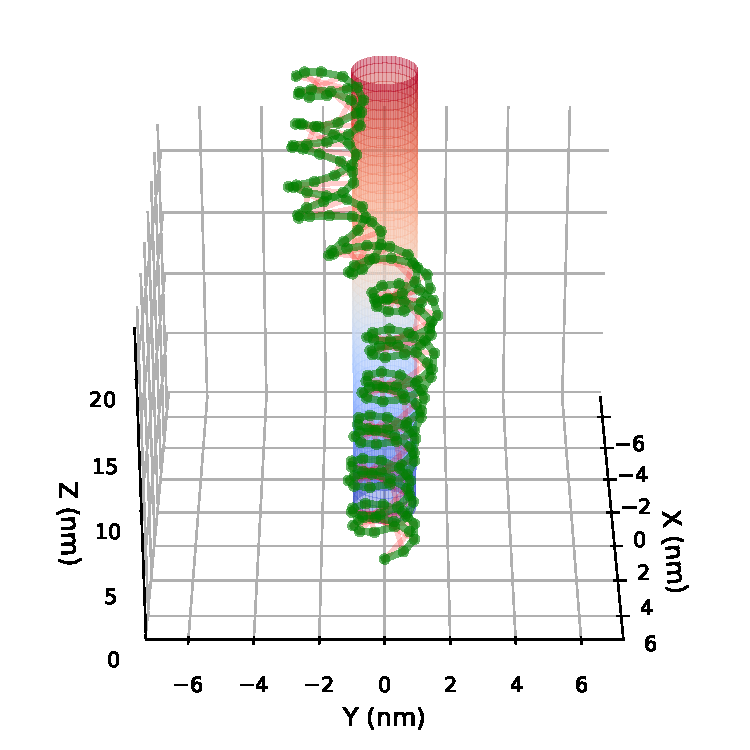
\includegraphics[width=\textwidth]{r2_A_2000000_16.pdf}
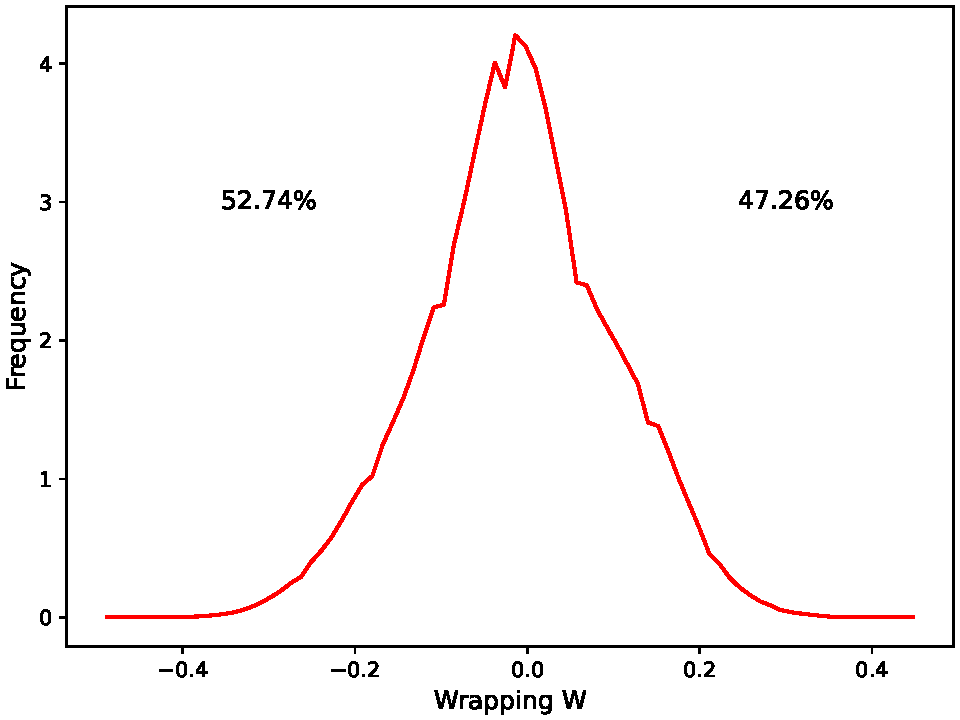
\includegraphics[width=\textwidth]{r2_A_wr_pr.pdf}
\caption{$\sigma_{rod}=$ \SI{2.1}{\nm}}
\label{fig:r2_a}
\end{subfigure}
\begin{subfigure}{.3\textwidth}
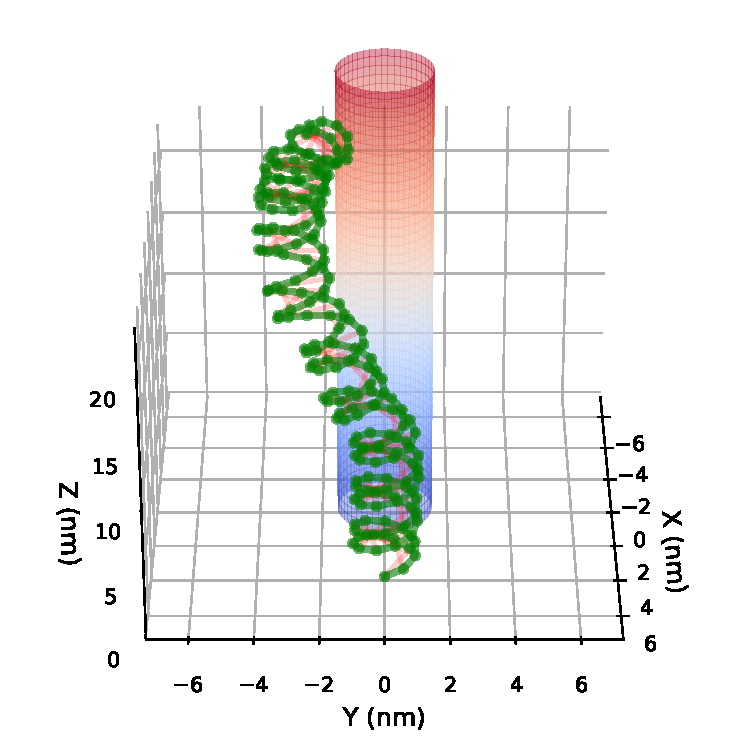
\includegraphics[width=\textwidth]{r2_B_2000000.pdf}
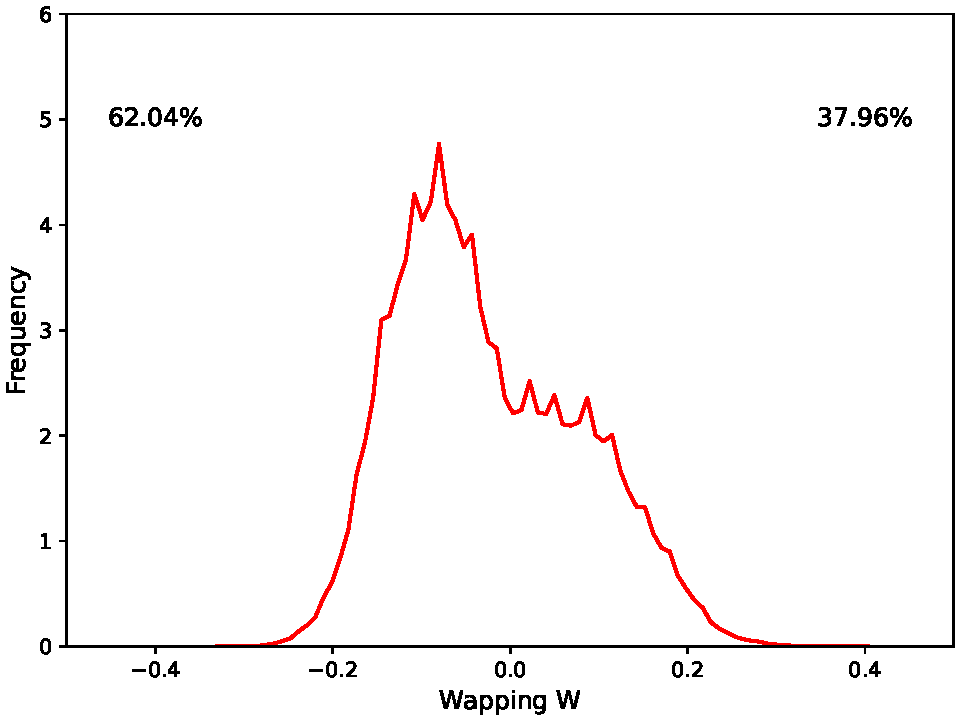
\includegraphics[width=\textwidth]{r2_B_wr_pr.pdf}
\caption{$\sigma_{rod}=$ \SI{3.1}{\nm}}
\label{fig:r2_b}
\end{subfigure}
\begin{subfigure}{.3\textwidth}
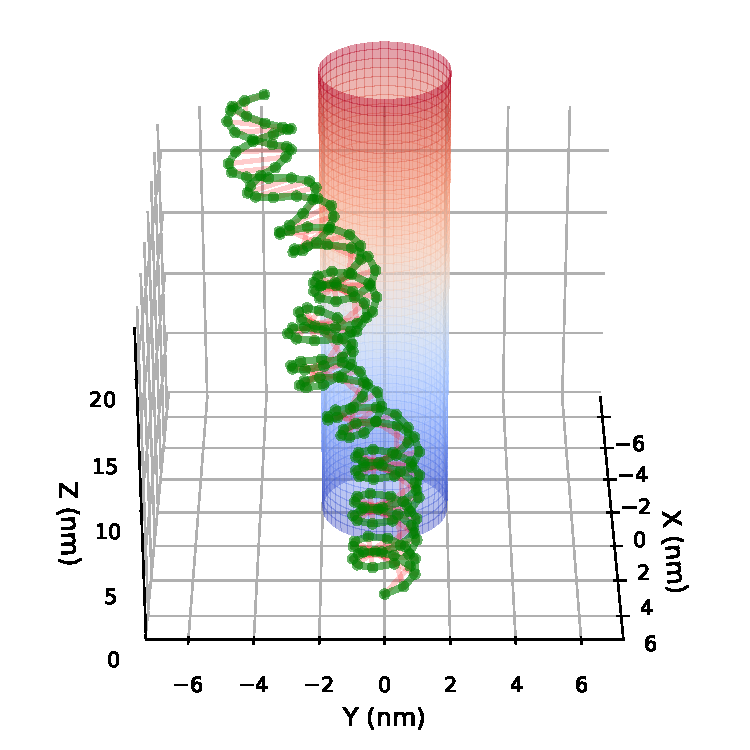
\includegraphics[width=\textwidth]{r2_C_2000000_18.pdf}
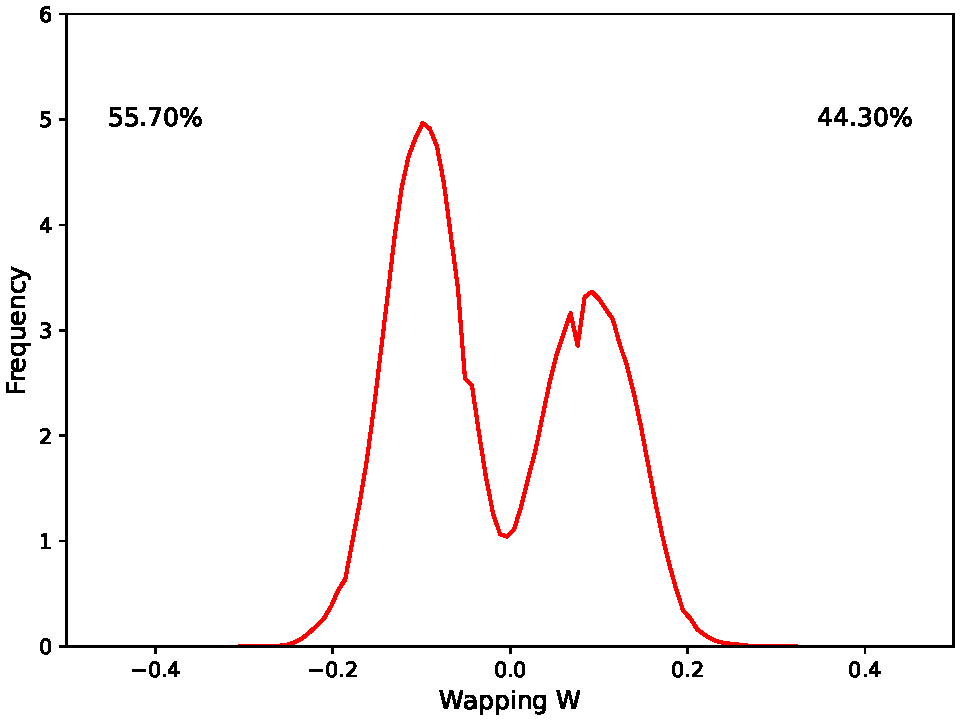
\includegraphics[width=\textwidth]{r2_C_wr_pr.pdf}
\caption{$\sigma_{rod}=$ \SI{4.1}{\nm}}
\label{fig:r2_c}
\end{subfigure}
\caption{Example of the DNA wrapping model (above) and probability distribution of the wrapping number obtained from $20$ Monte Carlo simulations of $2\times 10^6$ steps (down) with $\sigma_{rod}=$ \SI{2.1}{\nm} (a), \SI{3.1}{\nm} (b), and \SI{4.1}{\nm} (c). The rod global potential was used (Eq.~\ref{eq:rod_2}).}
\label{fig:r2}
\end{figure}

\subsection{Chiral selection in crossover and braiding of two juxtaposed DNA molecules}\label{sec:braF}
The above results (Sec.~\ref{sec:core} and~\ref{sec:rod}) indicate that DNA may have a preferred chirality for crossover and braiding due to its asymmetric elasticity.
Recent works indicate that right-handed crossover and left-handed braiding are preferable for two juxtapose DNA molecules in solution on the presence of cations~\cite{br_1, br_2, br_3, br_4, br_5}.
It should be noted that crossover and braiding are intimately correlated, since if one is right-handed the second is left-handed and vice versa.
The cited works have highlighted the electrostatic effects and steric effects: in the paper that I analyse they have investigated the roles of asymmetric elasticity.

Suppose there are two DNA molecules, A and B: they have modeled the attractive interaction and the excluded volume effect between these DNA molecules at the same time using the Morse potential for simplicity:
\begin{equation}\label{eq:ext}
V_{ext}^{AB}=\sum_{i=1}^{N}\sum_{j=1}^{N}D_{DNA}\left \{\exp\left [-2\beta_{DNA}\left (\left |\textbf{r}_{i}^{A}-\textbf{r}_{j}^{B}\right |-\sigma_{DNA}\right )\right ]-2\exp\left [-\beta_{DNA}\left (\left |\textbf{r}_{i}^{A}-\textbf{r}_{j}^{B}\right |-\sigma_{DNA}\right )\right ]\right \}
\end{equation}
where $\textbf{r}_{i}^{A}$ and $\textbf{r}_{j}^{B}$ represent the positions of $i$-th and $j$-th nodal point of the two DNA models.
The parameter $\sigma_{DNA}$ is the equilibrium distance between the nodal points of the two molecules and they have set it to \SI{2.1}{\nm}.
$\beta_{DNA}=$ \SI{0.8}{\per\nm} determines the width of the Morse potential, while $D_{DNA}$ determines the strength of the DNA-DNA interaction.
It should be noted that the potential of Eq.~\ref{eq:ext} is global as Eq.~\ref{eq:rod_2}.

Eq.~\ref{eq:ext} represent the attraction potential between the two molecules due to salt condition, but there is also internal attraction inside the same molecule.
They have used Morse potential to describe this interaction, using the same parameters used in the external potential (Eq.~\ref{eq:ext})
\begin{equation}\label{eq:int}
V_{int}^{X}=\sum_{i=1}^{N-n}\sum_{j=i+n}^{N}D_{DNA}\left \{\exp\left [-2\beta_{DNA}\left (\left |\textbf{r}_{i}^{X}-\textbf{r}_{j}^{X}\right |-\sigma_{DNA}\right )\right ]-2\exp\left [-\beta_{DNA}\left (\left |\textbf{r}_{i}^{X}-\textbf{r}_{j}^{X}\right |-\sigma_{DNA}\right )\right ]\right \}
\end{equation}
where the superscript $X$ distinguishes the two DNA molecules $\left (X=\left \{A,\ B\right \}\right )$.
They have set $n=7$ to remove the repulsions between very close nodal points in comparison to $\sigma_{DNA}$.
This potential does not break the symmetry between left- and right-handed crossovers and braidings.

In order to characterize chirality and degree of braiding they have introduced braiding number
\begin{equation}\label{eq:braiding}
B=\dfrac{1}{2\pi}\sum_{i=1}^{N-1}sgn\left [\left (\textbf{C}_{i+1}-\textbf{C}_{i}\right )\cdot\left (\textbf{B}_{i}\times\textbf{B}_{i+1}\right )\right ]\sin^{-1}\left (\left |\textbf{B}_{i}\times\textbf{B}_{i+1}\right |\right )
\end{equation}
where
\begin{equation}
\textbf{C}_{i}=\dfrac{\textbf{r}_{i}^{A}+\textbf{r}_{i}^{B}}{2},\qquad \textbf{B}_{i}=\dfrac{\textbf{r}_{i}^{A}-\textbf{r}_{i}^{B}}{\left |\textbf{r}_{i}^{A}-\textbf{r}_{i}^{B}\right |}
\end{equation}
Positive values of $B$ signify right-handed braiding, while absolute value is a measure of the number of braiding turns.
Because of the global attractions between and within the DNA model molecules, the two segments can sometimes collapse and form a globe.
To regularize this aspect, they have introduced a stretch force on the z-axis
\begin{equation}\label{eq:ten}
V_{ten}^{A}=-Fz_{N}^{A},\qquad V_{ten}^{B}=-Fz_{N}^{B}
\end{equation}
where $z_{N}^{X}$ is the z-coordinate of the last nodal point of the $X$ molecule.
The parameter $F$ is the force, and I have set it to \SIlist{0; 20; 40; 60; 80; 100}{\pico\newton}.
I perform Monte Carlo simulations for two DNA molecules, each with $N=100$ nodes and using for Eq.~\ref{eq:prob} this total energy
\begin{equation}\label{eq:bra_energy}
V=V_{bond}+V_{bend}+V_{ext}^{AB}+V_{int}^{A}+V_{int}^{B}+V_{ten}^{A}+V_{ten}^{B}
\end{equation}

The initial conformation is two straight molecules along the z-axis, with $\textbf{r}_{1}^{A}=\left (0,\ 0,\ 0\right )^T$ and $\textbf{r}_{1}^{B}=\left (4,\ 0,\ 0\right )^T$ in unit of \si{\nm}.
Fig.~\ref{fig:braF} shows examples of conformations (top), braiding number (Eq.~\ref{eq:braiding}) (middle), and probability distribution of the braiding number (bottom) in $20$ Monte Carlo simulation of $2\times 10^6$ steps, discarding the first $2\times 10^5$.
$D_{DNA}$ is set to \SI{0.7}{\pico\newton\nano\meter}.
The $F$ parameter is set to \SI{0}{\pico\newton} in Fig.~\ref{fig:braF_a}, \SI{60}{\pico\newton} in Fig.~\ref{fig:braF_b}, and \SI{100}{\pico\newton} in Fig.~\ref{fig:braF_c}.

From Fig.~\ref{fig:braF_a} (middle) -when there is not stretch force- the braiding number mostly takes negative values, indicating that the left-handed braiding is preferred in this simulation.
Introducing the stretch force -let's see Fig.~\ref{fig:braF_b} and~\ref{fig:braF_c}- we see that the absolute values of $B$ tend to decrease as the tension increases.
This means that DNA molecules do not braid largely, but just crossover.
However they still prefer negative $B$ conformations that, since the conventions about crossover~\cite{br_1}, implies right-handed crossover.

Looking at the down parts of Fig.~\ref{fig:braF} we observe the probability distribution of braiding number.
When $F=$ \SI{0}{\pico\newton} (Fig.~\ref{fig:braF_a}) the probability is distributed over a wide range, with some peaks in both negative and positive ranges but still with higher probability for negative values.
With $F=$ \SI{60}{\pico\newton} (Fig.~\ref{fig:braF_b}) the probability is narrower than that of Fig.~\ref{fig:braF_a}.
It indicates, as said above, that the stretch force reduces the braiding, but it is still biased towards negative values.
There are two faint second peaks, one negative and one positive, that indicate semi-equilibrium conformations.
Fig.~\ref{fig:braF_c} shows braiding probability distribution when $F=$ \SI{100}{\pico\newton}.
The distribution is even narrower and symmetric, but we can still see the negative bias.

\begin{figure}[tb]
\centering
\begin{subfigure}{.3\textwidth}
\vspace{1.13cm}
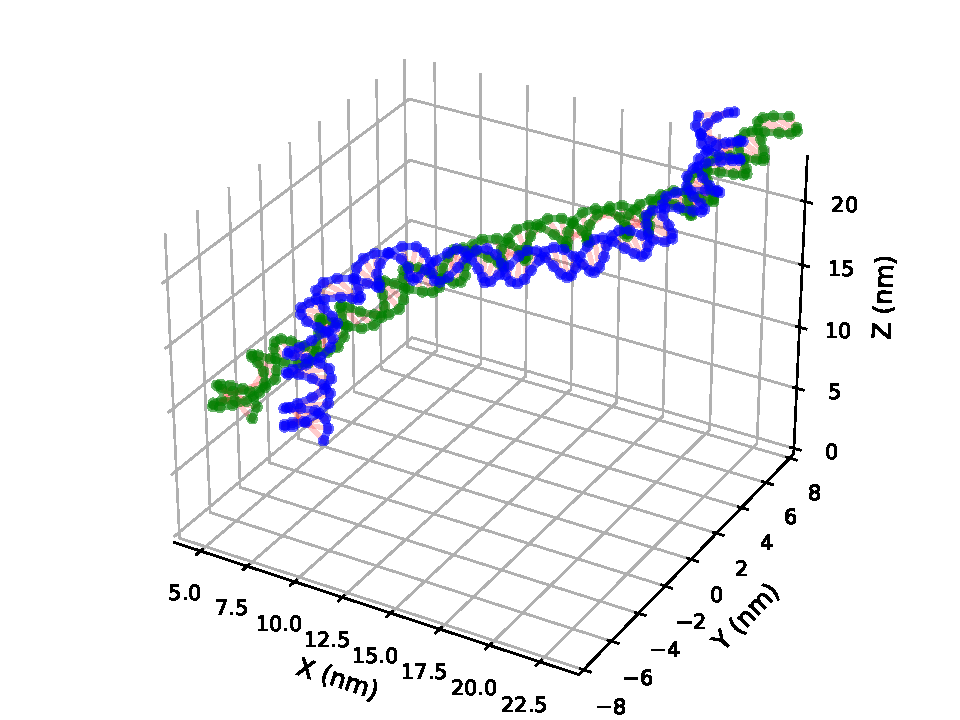
\includegraphics[width=\textwidth]{brF_0_2000000.pdf}
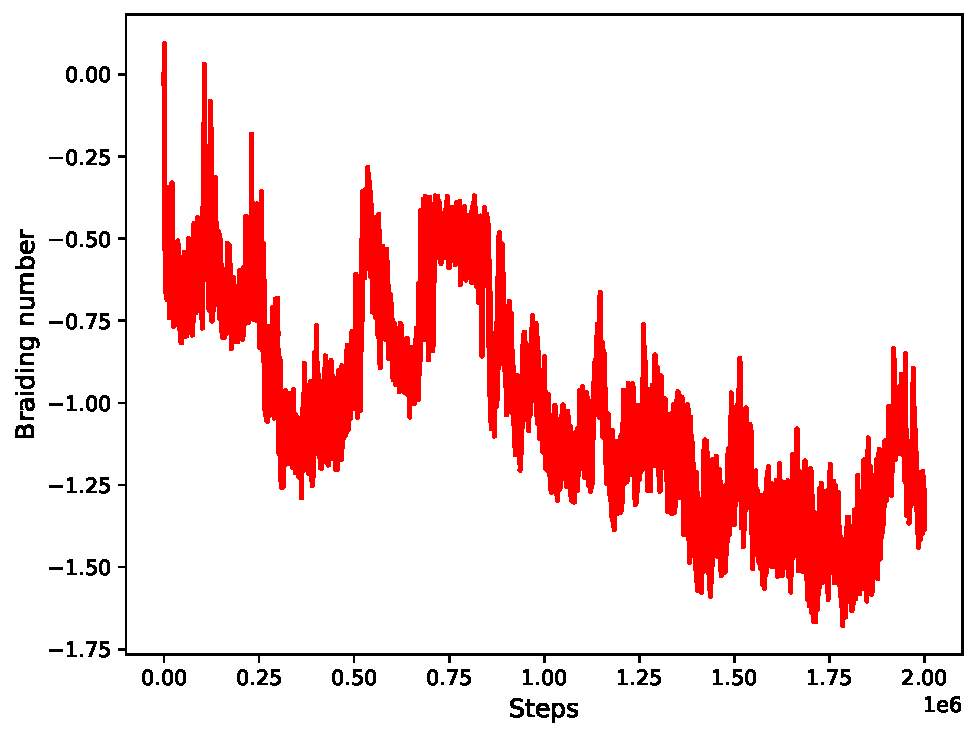
\includegraphics[width=\textwidth]{brF_0_braid.pdf}
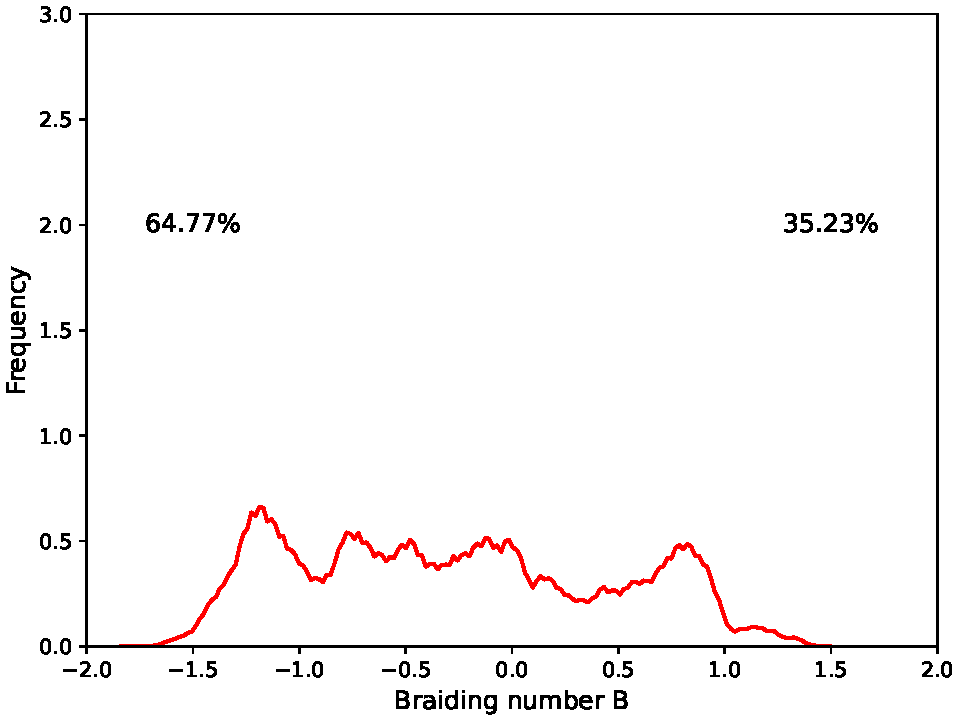
\includegraphics[width=\textwidth]{brF_0_br_pr.pdf}
\caption{$F=$ \SI{0}{\pico\newton}}
\label{fig:braF_a}
\end{subfigure}
\begin{subfigure}{.3\textwidth}
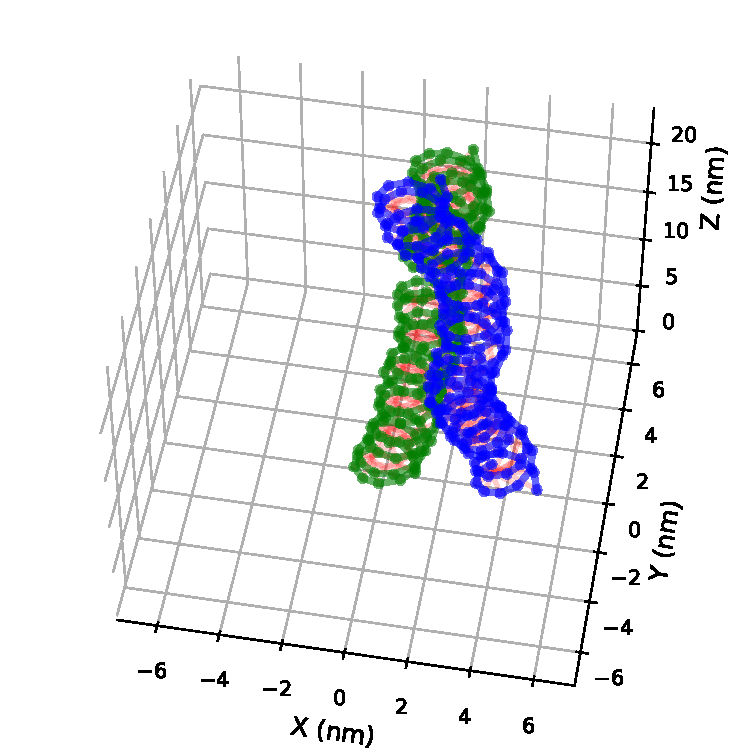
\includegraphics[width=\textwidth]{brF_60_2000000.pdf}
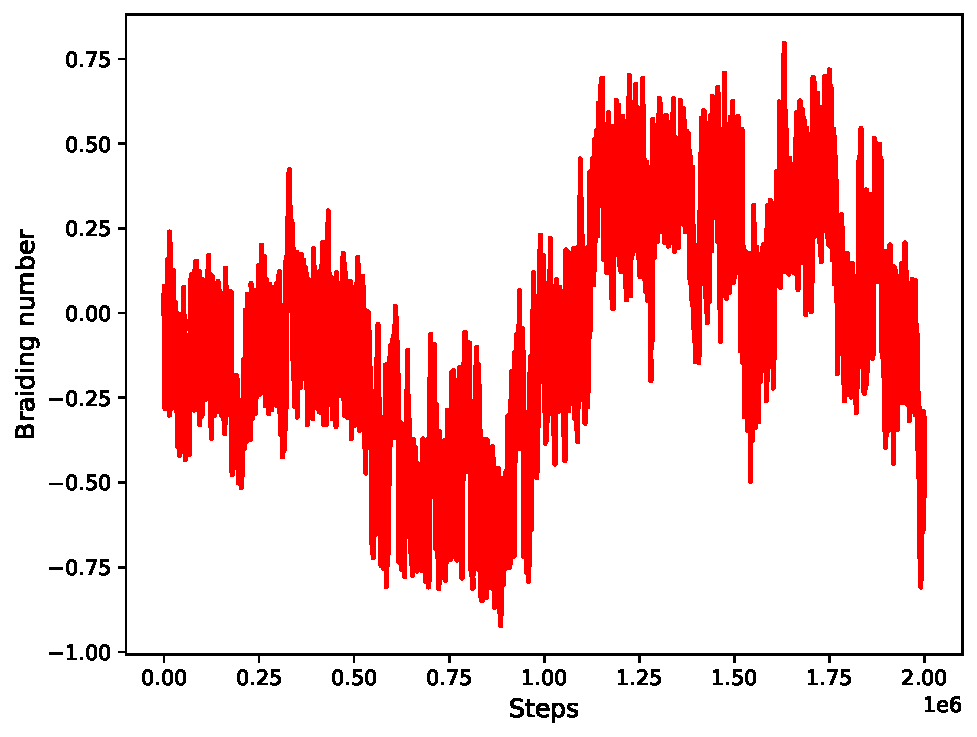
\includegraphics[width=\textwidth]{brF_60_braid.pdf}
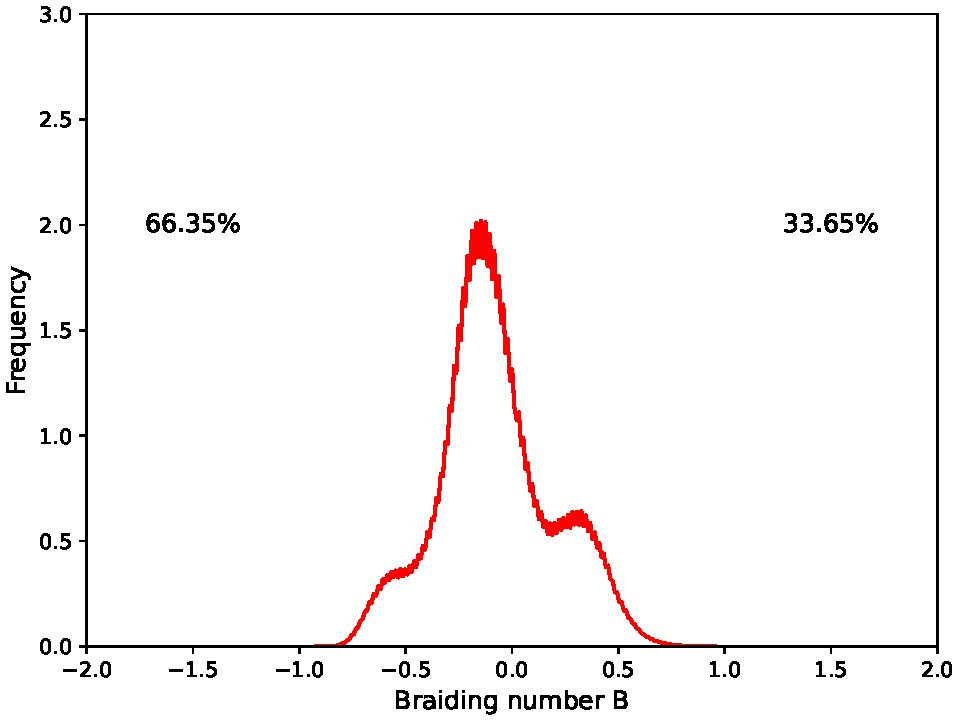
\includegraphics[width=\textwidth]{brF_60_br_pr.pdf}
\caption{$F=$ \SI{60}{\pico\newton}}
\label{fig:braF_b}
\end{subfigure}
\begin{subfigure}{.3\textwidth}
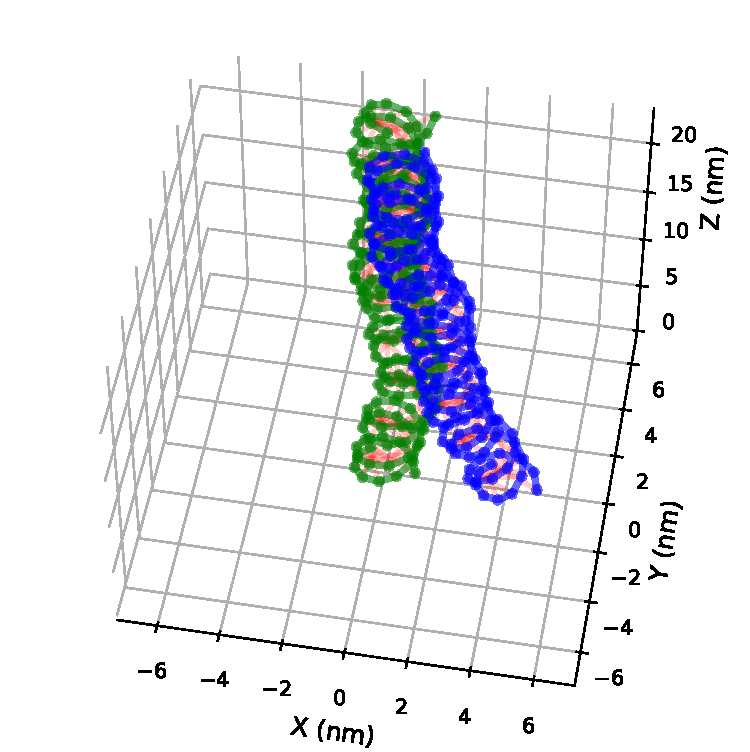
\includegraphics[width=\textwidth]{brF_100_2000000.pdf}
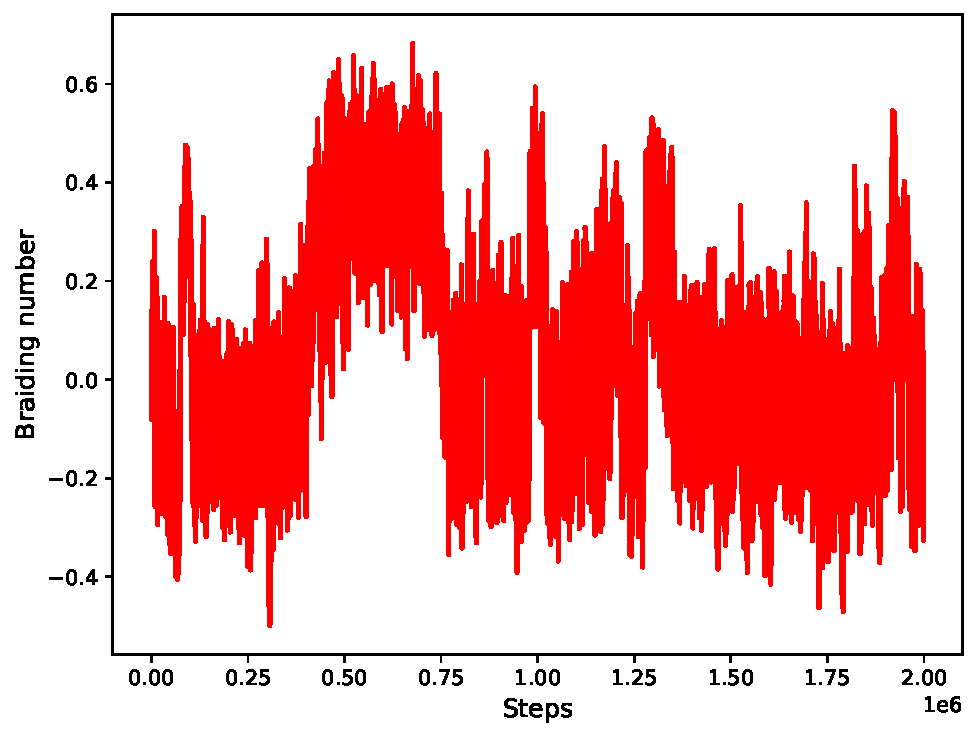
\includegraphics[width=\textwidth]{brF_100_braid.pdf}
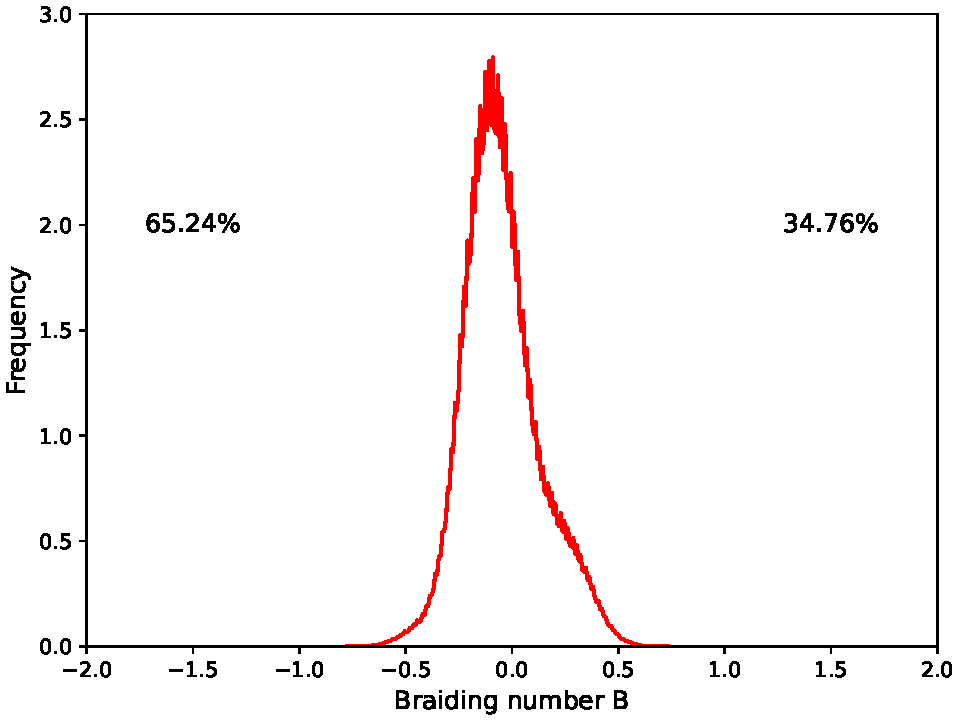
\includegraphics[width=\textwidth]{brF_100_br_pr.pdf}
\caption{$F=$ \SI{100}{\pico\newton}}
\label{fig:braF_c}
\end{subfigure}
\caption{Examples of the two DNA crossover model (above), evolution of braiding number of Eq.~\ref{eq:braiding} (middle), and probability distribution of braiding number obtained from $20$ Monte Carlo simulations of $2\times 10^6$ steps (down) with $F$ equal to \SI{0}{\pico\newton} (a), \SI{60}{\pico\newton} (b), and \SI{100}{\pico\newton} (c).}
\label{fig:braF}
\end{figure}

Fig.~\ref{fig:braF_pr} summarizes the dependence of the probabilities for left-handed braiding and that for right-handed braiding on the magnitude of tension $F$.
The probabilities are defined as the integrated areas of the probability distributions as in Fig~\ref{fig:braF} over the range $B<0$ and $B>0$.
The increasing symmetry respect negative and positive values of braiding number is not so clear and there are more fluctuations than in the original paper.

\begin{figure}[tb]
\centering
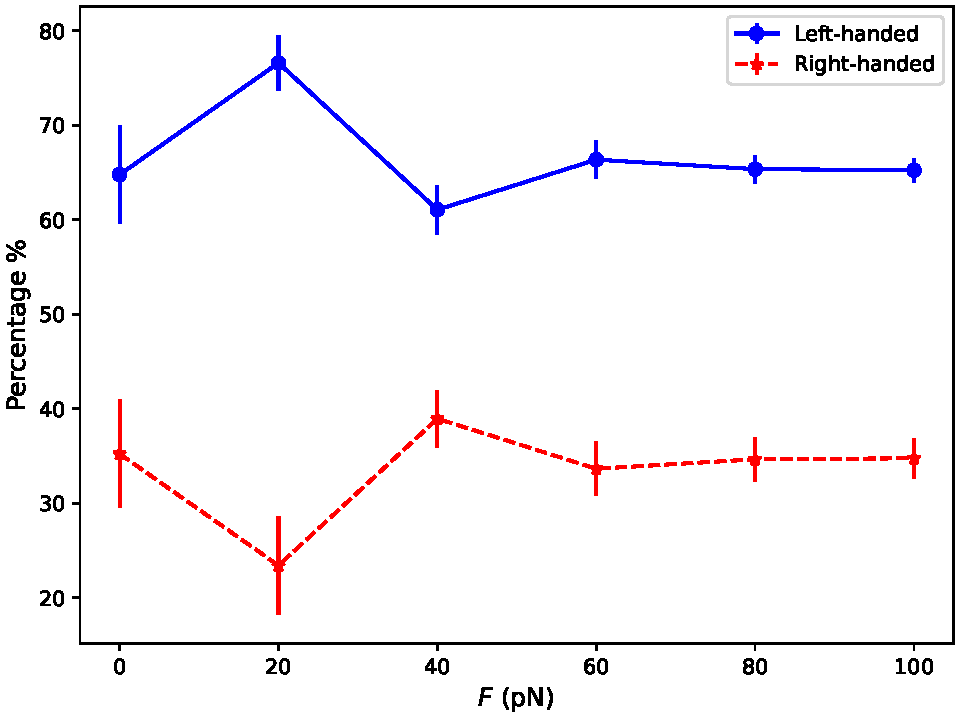
\includegraphics[width=.5\textwidth]{brF_br_gr.pdf}
\caption{Dependence of the probabilities for left- and right-handed braiding of a pair of DNA model molecules on tension $F$.
Blue circles -solid line- represent the probability for the left-handed braiding, while red squares -broken line- represent the probability for right-handed braiding.
Error bars represent standard error.}
\label{fig:braF_pr}
\end{figure}

\subsection{Dependence of braiding chirality on the strength of DNA-DNA interaction}
Dependence of braiding behaviours on the strength of the interaction between DNA molecules is an interesting issue, since it can change significantly in solution depending on salt condition.
I study the previous energy equation (Eq.~\ref{eq:bra_energy}) changing $D_{DNA}$ parameter.
The simulations characteristics are the same as the previous ones made in Sec.~\ref{sec:braF}, setting $F=$ \SI{40}{\pico\newton}.

Fig.~\ref{fig:braD} shows examples of conformations (above), braiding number (Eq.~\ref{eq:braiding}) (middle), and probability distribution of the braiding number (down) in $20$ Monte Carlo simulation of $2\times 10^6$ steps, discarding the first $2\times 10^5$.
The $D_{DNA}$ parameter is set to \SI{0.5}{\pico\newton\nano\meter} in Fig.~\ref{fig:braD_a}, \SI{1.0}{\pico\newton\nano\meter} in Fig.~\ref{fig:braD_b}, and \SI{1.5}{\pico\newton\nano\meter} in Fig.~\ref{fig:braD_c}.
When the interaction is weaker as in Fig.~\ref{fig:braD_a}, the braiding number switches between positive and negative values during a single Monte Carlo simulation.
When the interaction becomes stronger as in Fig.~\ref{fig:braD_b}, frequency of switching decreases, but the absolute value of the braiding number can become larger, and usually tends to assume negative values.
When the attractive interaction becomes even stronger as in Fig.~\ref{fig:braD_c}, the switching between left- and right-handed braiding hardly occurs during a single Monte Carlo simulation.

Watching the probabilities distributions, when the interaction is weak as in Fig.~\ref{fig:braD_a}, the distribution is narrow and with a single peak: this shows that the DNAs do not braiding, just crossover.
However it is already biased towards negative values.
When the attractive interaction increases as in Fig.~\ref{fig:braD_b}, the distribution becomes wider and is still biased towards negative values, with more peaks.
Multiple negative peaks are due to the tendency of the model to increase the contacts at the expense of bending energy, which is in turn due to the string attraction.
When the interaction becomes stronger as in Fig.~\ref{fig:braD_c}, the distribution becomes even wider in negative and positive region.
In this condition the two molecules can crossover even deeper and braid each other.
There are many peaks, indicating a stepwise braiding.
In the negative range, the distribution is biased towards peaks with greater absolute values, while in the positive region it is biased towards low peaks.
This means that the left-handed braiding tends to have larger number of braiding turns than right-handed one.

\begin{figure}[tb]
\centering
\begin{subfigure}{.3\textwidth}
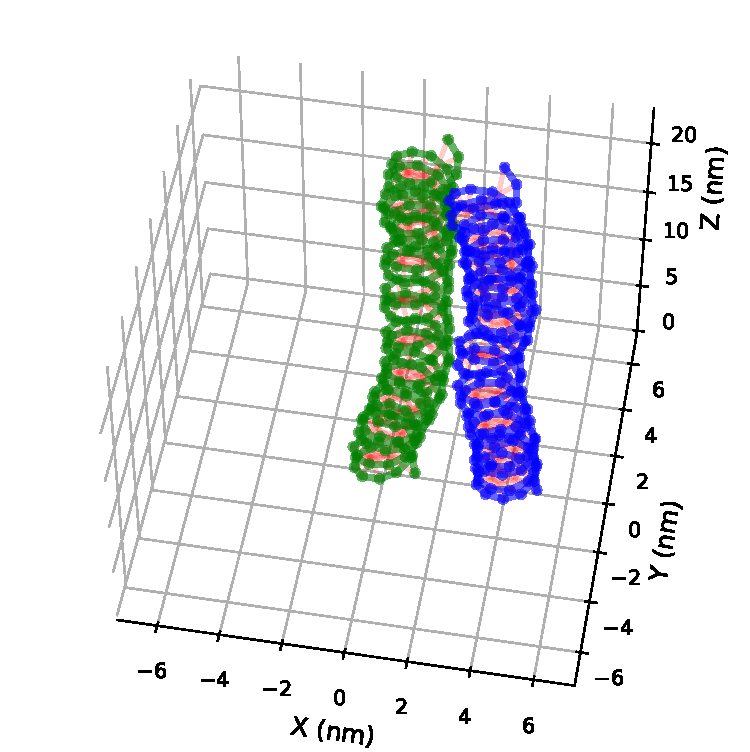
\includegraphics[width=\textwidth]{brD_5_2000000.pdf}
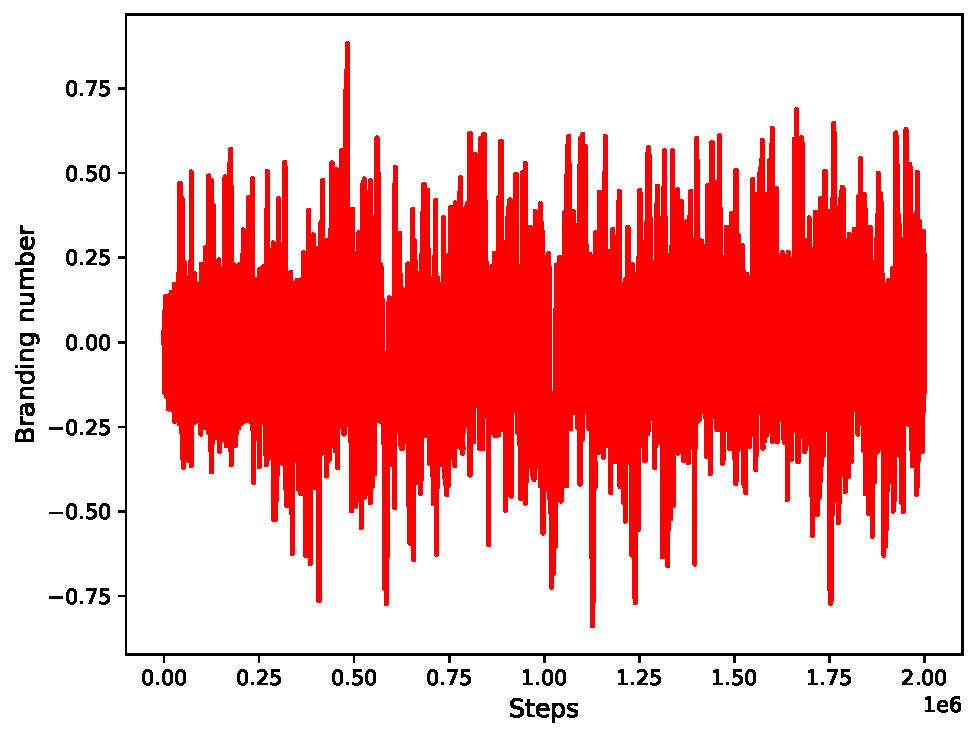
\includegraphics[width=\textwidth]{brD_5_brand.pdf}
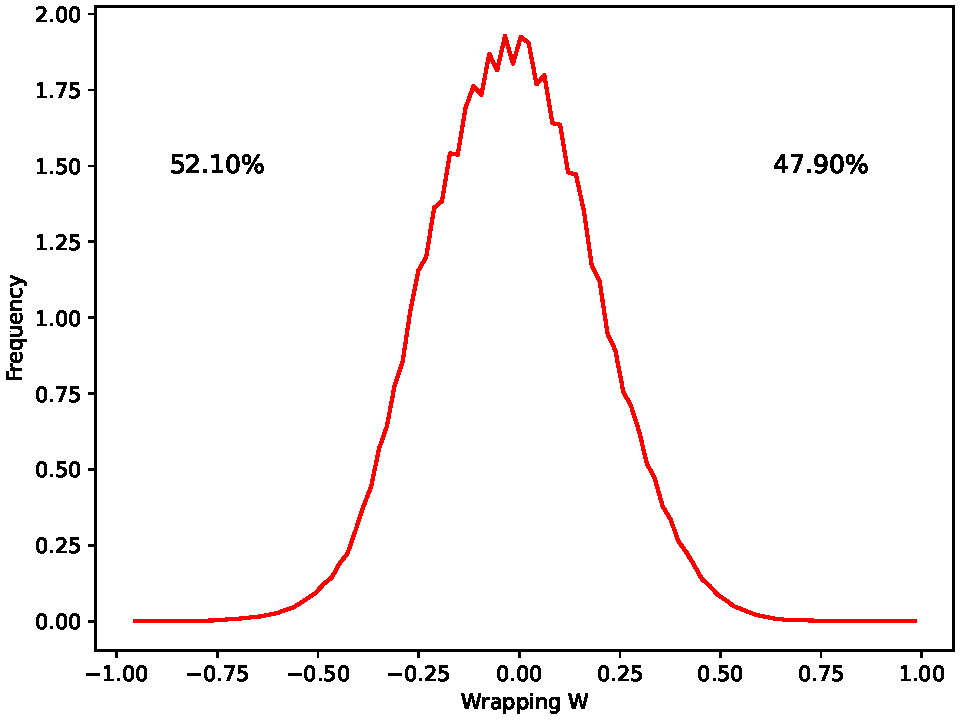
\includegraphics[width=\textwidth]{brD_5_br_pr.pdf}
\caption{$D_{DNA}=$ \SI{0.5}{\pico\newton\nano\meter}}
\label{fig:braD_a}
\end{subfigure}
\begin{subfigure}{.3\textwidth}
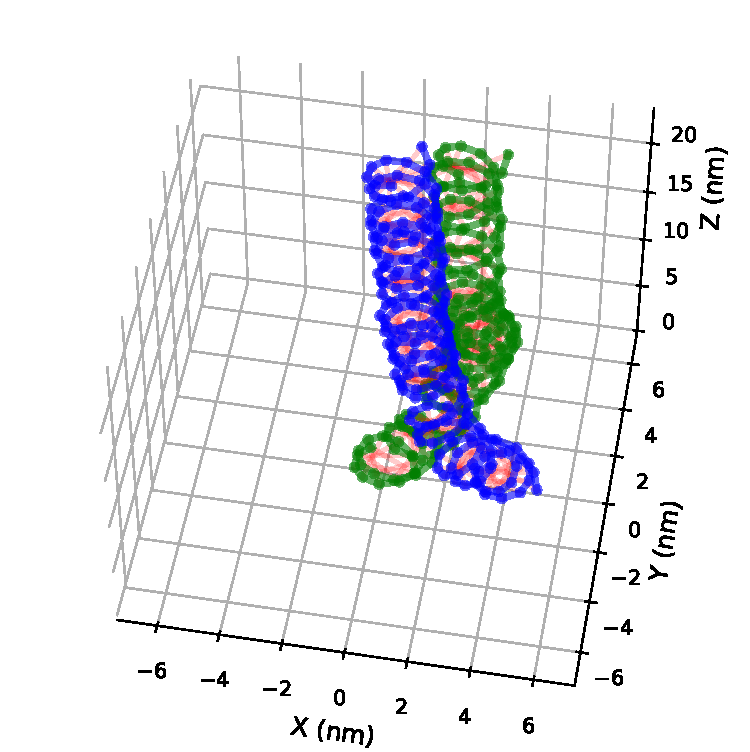
\includegraphics[width=\textwidth]{brD_100_2000000.pdf}
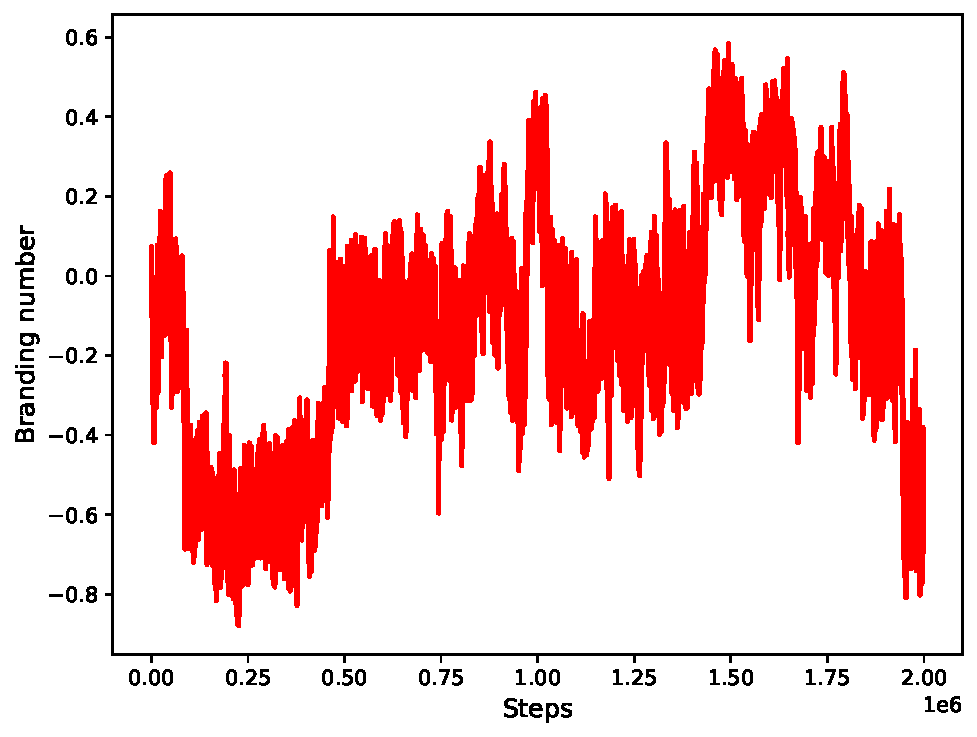
\includegraphics[width=\textwidth]{brD_100_brand.pdf}
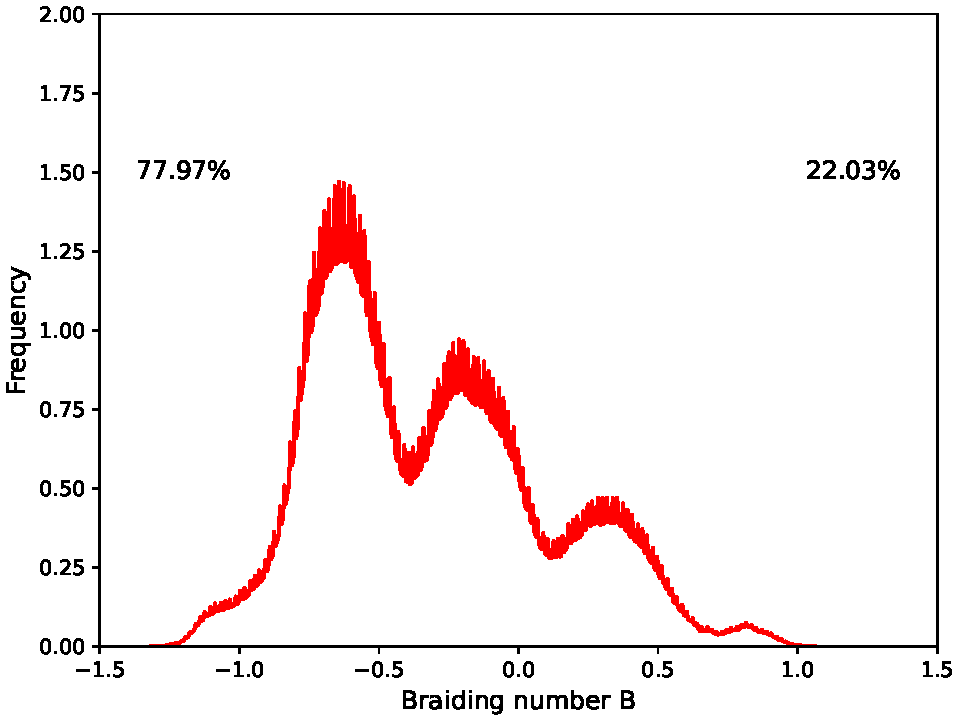
\includegraphics[width=\textwidth]{brD_100_br_pr.pdf}
\caption{$D_{DNA}=$ \SI{1.0}{\pico\newton\nano\meter}}
\label{fig:braD_b}
\end{subfigure}
\begin{subfigure}{.3\textwidth}
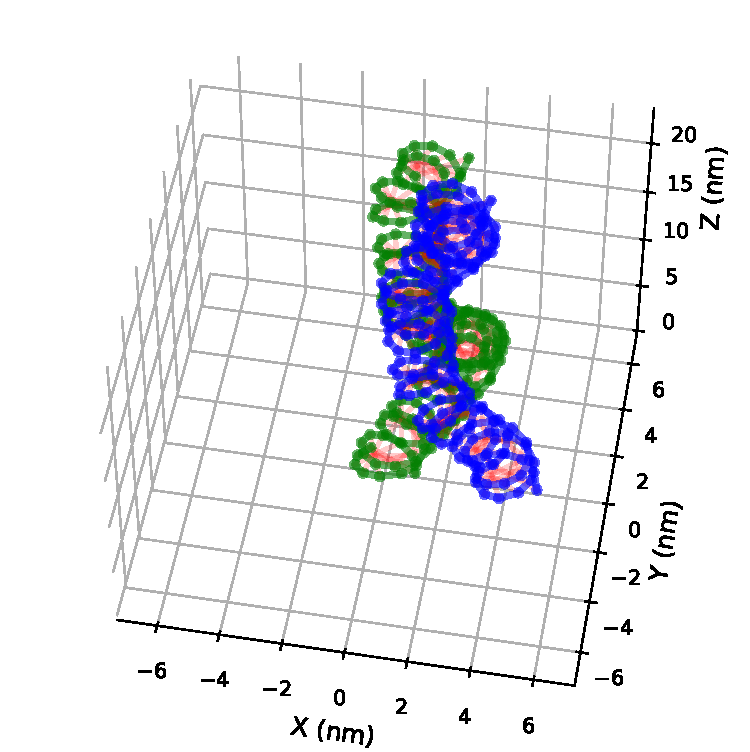
\includegraphics[width=\textwidth]{brD_150_2000000.pdf}
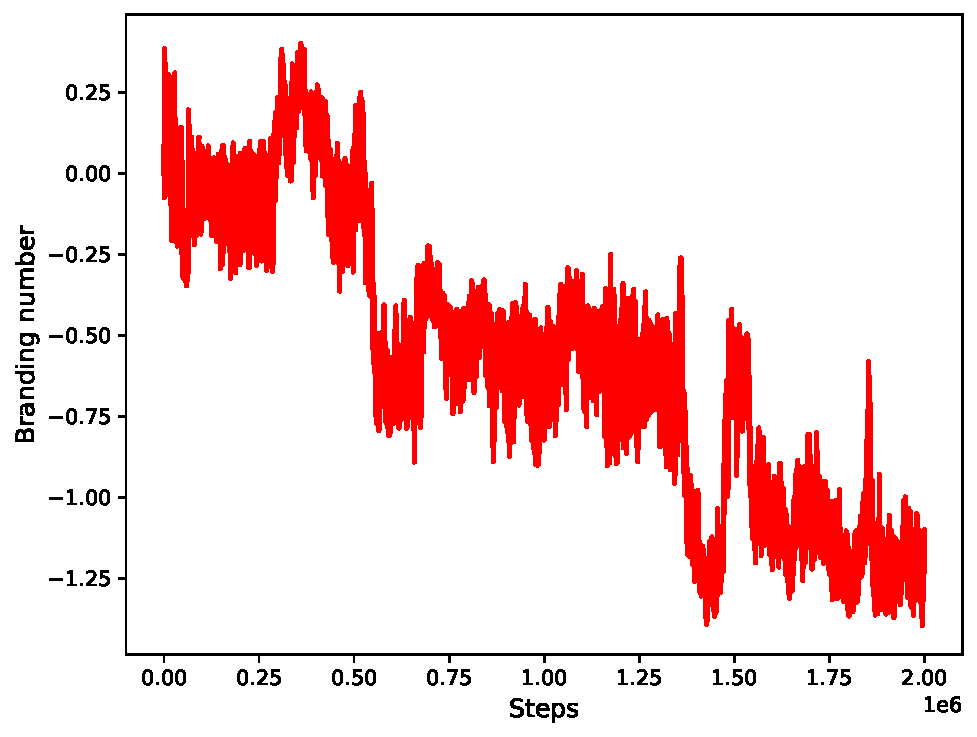
\includegraphics[width=\textwidth]{brD_150_brand.pdf}
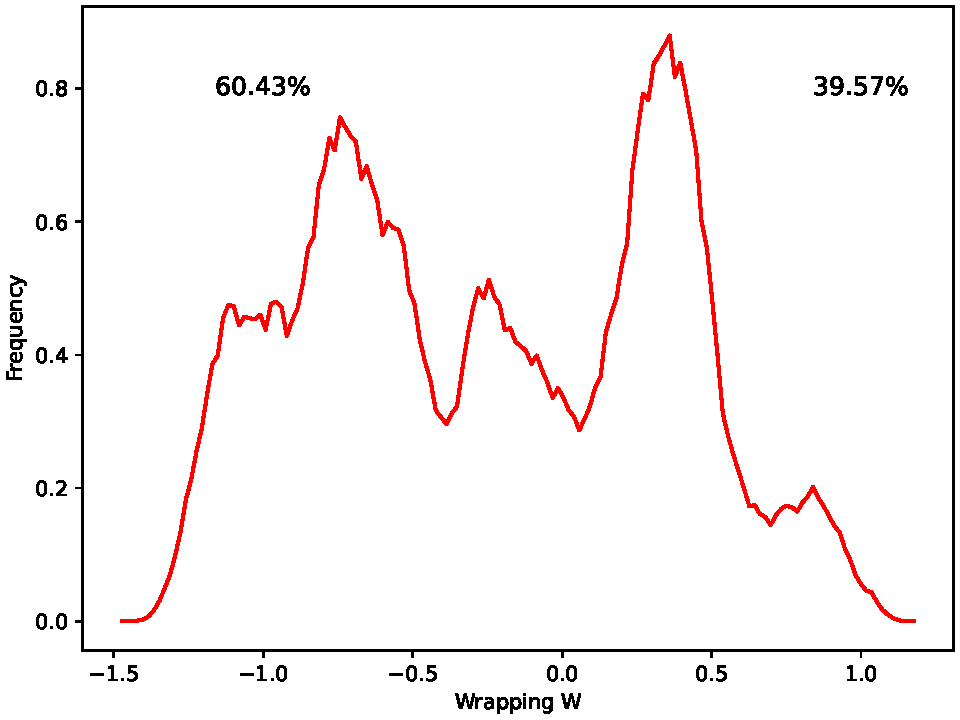
\includegraphics[width=\textwidth]{brD_150_br_pr.pdf}
\caption{$D_{DNA}=$ \SI{1.5}{\pico\newton\nano\meter}}
\label{fig:braD_c}
\end{subfigure}
\caption{Examples of the two DNA crossover model (above), evolution of braiding number of Eq.~\ref{eq:braiding} (middle), and probability distribution of braiding number obtained from $20$ Monte Carlo simulations of $2\times 10^6$ steps (down) with $D_{DNA}$ equal to \SI{0.5}{\pico\newton\nano\meter} (a), \SI{1.0}{\pico\newton\nano\meter} (b), and \SI{1.5}{\pico\newton\nano\meter} (c).}
\label{fig:braD}
\end{figure}

We see that braiding number is mostly negative, and it spreads more values increasing the DNA-DNA interaction parameter ($D_{DNA}$).
Additionally, the left-handed braiding probability increases as the interaction parameter increases for small value; then decreases as the increasing of $D_{DNA}$, as can be see in Fig.~\ref{fig:braD_pr}.

\begin{figure}[tb]
\centering
\includegraphics[width=.5\textwidth]{brD_br_gr.pdf}
\caption{Dependence of the probabilities for left- and right-handed braiding of a pair of DNA model molecules on DNA-DNA attractive interaction $D_{DNA}$.
Blue circles -solid line- represent the probability for the left-handed braiding, while red squares -broken line- represent the probability for right-handed braiding.
Error bars represent standard error.}
\label{fig:braD_pr}
\end{figure}

\section{Conclusions}
I have followed the studied paper that had investigated the elastic mechanisms of the selection of chirality in DNA wrapping, crossover, and braiding based on a coarse-grained model and I have tried to reproduce their results.

The DNA model consisted of two elastic chains mutually intertwine in a right-handed manner forming a double-stranded helix with a distinction between major and minor grooves.
The model has been inclined to writhe to the left direction, even if the potential does not have an asymmetric term: this has been a consequence of the right-handed helix.
The left-handed wrapping has been statistically preferred around a spherical core particle and an uniform rod.
Monte Carlo simulations have suggested that two juxtaposed DNA molecules could braid each other spontaneously under moderate attractive interactions preferring left-handed braiding.

Overall my simulations have reproduced their results, but in some cases there have been some discrepancies.
The peaks that I have found in probability distributions of wrapping number $W$ and braiding number $B$ are not the same founded in the paper.
This suggest that the potential landscape has not been so regular and there have been plenty of attractive conformations that the model could take on.
The biggest discrepancy regards Fig.~\ref{fig:braF_pr}.
In the paper the left-handed probability has decreased as the force has increased; in my simulations the behaviour has not been so clear and there have been more fluctuations and irregularities.

The study has highlighted almost exclusively the roles of asymmetric bend-writhe elasticity of DNA in the formation of higher-order structures, but it has some limitations.
It has used limited degrees of freedom, e.i. bending, dihedral and twist angles, but in reality other internal degrees of freedom could also couple each other giving rise to more complex behaviours.
In addition, the constant used to determine bonding and bending energy (Eq.~\ref{eq:bond} and~\ref{eq:bend}), $K_{bond}$ and $K_{bend}$ have been determined to approximate as better as they could the bending persistence length  of real DNA, but they could be better evaluated through other experiments and analysis about energy.
Almost all the energy potential have been Morse potential: in reality the Coulomb potential had been the correct one, but it would have been too computational expensive.

\clearpage
\addcontentsline{toc}{section}{\refname}
\printbibliography
\end{document}
